\documentclass[17pt]{beamer}
%\documentclass[handout]{beamer} %Makes Handouts
\usetheme{Singapore} %Gray with fade at top
\useoutertheme[subsection=false]{miniframes} %Supppress subsection in header
\useinnertheme{rectangles} %Itemize/Enumerate boxes
\usecolortheme{seagull} %Color theme
\usecolortheme{rose} %Inner color theme

\definecolor{light-gray}{gray}{0.75}
\definecolor{dark-gray}{gray}{0.55}
\setbeamercolor{item}{fg=light-gray}
\setbeamercolor{enumerate item}{fg=dark-gray}

\setbeamertemplate{navigation symbols}{}
\setbeamertemplate{mini frames}{}
%\setbeamercovered{dynamics}
\setbeamerfont*{title}{size=\Large,series=\bfseries}
\setbeamerfont{footnote}{size=\tiny}

%\setbeameroption{notes on second screen} %Dual-Screen Notes
%\setbeameroption{show only notes} %Notes Output

\setbeamertemplate{frametitle}{\vspace{.5em}\bfseries\insertframetitle}
\newcommand{\heading}[1]{\noindent \textbf{#1}\\ \vspace{1em}}
\newcommand{\questions}{\frame{{\large Questions?}}}

\usepackage{bbding,color,multirow,times,ccaption,tabularx,graphicx,verbatim,booktabs}
\usepackage{colortbl} %Table overlays
\usepackage[english]{babel}
\usepackage[latin1]{inputenc}
\usepackage[T1]{fontenc}
\usepackage{lmodern}
\usepackage{alltt}

\usepackage{tikz}
\usetikzlibrary{shapes,arrows,decorations.pathreplacing,calc}


\author[]{Thomas J. Leeper}
\institute{
  Government Department\\London School of Economics and Political Science
}


\title{Session III\\External Validity}

\date[]{}

\begin{document}

\frame{\titlepage}

\frame{

\frametitle{Share your TESS Examples}

In groups of 4--5, share your TESS examples
\begin{itemize}
\item What was the researcher's question?
\item How did they test it experimentally?
\item What was interesting or surprising about the designs?
\end{itemize}

Take about 7--8 minutes.

}



\frame{\tableofcontents[subsubsectionstyle=hide]}

\section[External Validity]{External Validity of a Sample}
\frame{\tableofcontents[currentsection,subsubsectionstyle=hide]}

\frame{

\frametitle{Think--Pair--Share}

Consider the following question:

What makes an experiment (or any research study) generalizable? What does it mean for a study's results to ``generalize''?

\begin{enumerate}
\item Write or think to yourself for 90 seconds
\item Then, discuss with the person next to you
\end{enumerate}

}


\frame{
\frametitle{{\normalsize ``The Gold Standard''}}

\small
\textit{a population-based experiment uses survey sampling methods to produce a collection of experimental subjects that is representative of the target population of interest for a particular theory \dots the population represented by the sample should be representative of the population to which the researcher intends to extend his or her findings. In population-based experiments, experimental subjects are randomly assigned to conditions by the researcher}\\

\vspace{0.5em}
{\footnotesize p2. from Mutz, Diana. 2011. \textit{Population-Based Survey Experiments}. Princeton University Press.\par}

}


\frame{
	\frametitle{Surveys Start with an Inference Population}
	
	\small
	\begin{itemize}\itemsep0.25em
		\item We want to speak to a population
		\item But what population is it?
			\begin{itemize}
			\item<2-> A national population?
			\item<3-> Adults in Western, industrialized democracies?
			\item<4-> All human beings?
			\end{itemize}
		\item<5-> This is rarely specified, but is important when we think about whether a sample is appropriate
	\end{itemize}
}



\frame{
	\frametitle{A Hypothetical Census}

	\begin{itemize}\itemsep1em
		\item Advantages
			\begin{itemize}
				\item<2-> Perfectly representative
				\item<2-> Sample statistics are population parameters
			\end{itemize}
		\item Disadvantages
			\begin{itemize}
				\item<3-> Costs
				\item<3-> Feasibility
				\item<3-> Need
			\end{itemize}		
	\end{itemize}
}


\subsection{Design-based}
\frame{\tableofcontents[currentsection, currentsubsection, subsubsectionstyle=hide]}

\frame{

\frametitle{{\normalsize Sampling Considerations\dots}}

\small

\begin{itemize}\itemsep0.25em
\item Design-based survey samples all work from the premise of each unit having a \textit{known, non-zero} probability of being sampled
	\begin{itemize}\footnotesize
	\item SRS is representative per se
	\item Non-self-weighting samples representative when weighted
	\end{itemize}
\item<2-> Random sampling ensures that samples are, \textit{in expectation}, representative of the population \textit{in all respects}
	\begin{itemize}\footnotesize
	\item Demographics
	\item Covariances
	\item Potential outcomes
	\end{itemize}
\end{itemize}
}


\frame{}

\begin{frame}[plain]{}
\frametitle{Representativeness}

\vspace{0.25em}

What does it mean for a sample to be representative?

\begin{itemize}\small
	\item<2-> Census?
	\item<3-> Probability-based sampling?
	\item<4-> Quota fulfillment?
	\item<5-> Others?
\end{itemize}

\onslide<6->{Which of these matter?}
\end{frame}

% what kinds of representativeness do we care about?



\frame{

\frametitle{{\large Combining Probability Sampling and Experimental Design}}

\small

\begin{itemize}\itemsep0.2em
\item Sample is representative of population in every respect (in expectation)
\item Sample Average Treatment Effect (SATE) is the average of the sample's individual-level treatment effects
	\begin{itemize}\footnotesize
	\item Unbiased estimate of PATE
	\item Not necessarily any unit's individual treatment effect
	\item Blocking might reduce variance
	\item Optimized for estimating SATE
	\end{itemize}
\end{itemize}
}



\frame{

Credibility of all of this is based on \textit{design} only

\vspace{1em}

\onslide<2->{Sampling aspect only works in a world of perfect coverage and no response bias}

}

\frame<1-3>[label=myview]{
\frametitle{My View}

100\% design-based inference does not exist!

\small

\begin{itemize}\itemsep0.25em
\item<2-> All survey designs involve reweighting adjustments
\item<3-> Representativeness is a more complex issue than demographic comparisons
\item<4-> Randomization gives us clear causal inference about a \textit{local} effect
	\begin{itemize}
	\item Sacrifice representativeness for causal inference
	\item Try to figure nature of the \textit{localness}
	\end{itemize}
\end{itemize}
}




\frame{

\footnotesize
\begin{tabular}{ l r r r r r r r} \toprule\toprule
   & {\bf GfK} & {\bf Poll} & {\bf Student} & {\bf Staff}  & {\bf MTurk} & {\bf Ads} & {\bf ANES}\\ \midrule
{\bf Dem. (\%)}      & 51.3 & 86.1 & 75.7 & 66.4 & 62.1 & 72.1 & 46.2 \\  
{\bf Rep. (\%)}    & 46.0 &   7.7 & 17.8 & 16.4 & 20.3 &  14.7 & 39.3\\ 
{\bf Lib. (\%)}          & 27.8 & 75.4 & 68.5 & 62.7 & 60.4 & 66.2& 23.8\\
{\bf Con. (\%)} & 35.3 & 9.4 & 14.7 & 19.8 & 19.1 & 17.7& 36.1\\
{\bf Fem. (\%)}         & 51.1 & 60.8 & 56.4 & 50.8 & 41.7 & 65.3 & 51.9 \\
{\bf White (\%)}           & 77.9 & 67.6 & 62.9 & 60.2 & 76.0 & 53.8 & 80.4\\
{\bf Age}          & 49.4 & 40-49 & 18-24 & 25-34 & 25-34 & 25-34& 50-54 \\ 
{\bf Interest}       & 2.8 & 3.5 & 3.2 & 2.8 & 2.7 & 3.0 & 3.0\\ \midrule
{\bf N}                         & 593 & 741 & 299 & 128 & 1024 & 80&  -- \\ \bottomrule\bottomrule
\end{tabular}

\vspace{1em}

{\footnotesize Mullinix et al. 2015. ``The Generalizability of Survey Experiments.'' \textit{Journal of Experimental Political Science}.}
}

\frame{
\begin{center}
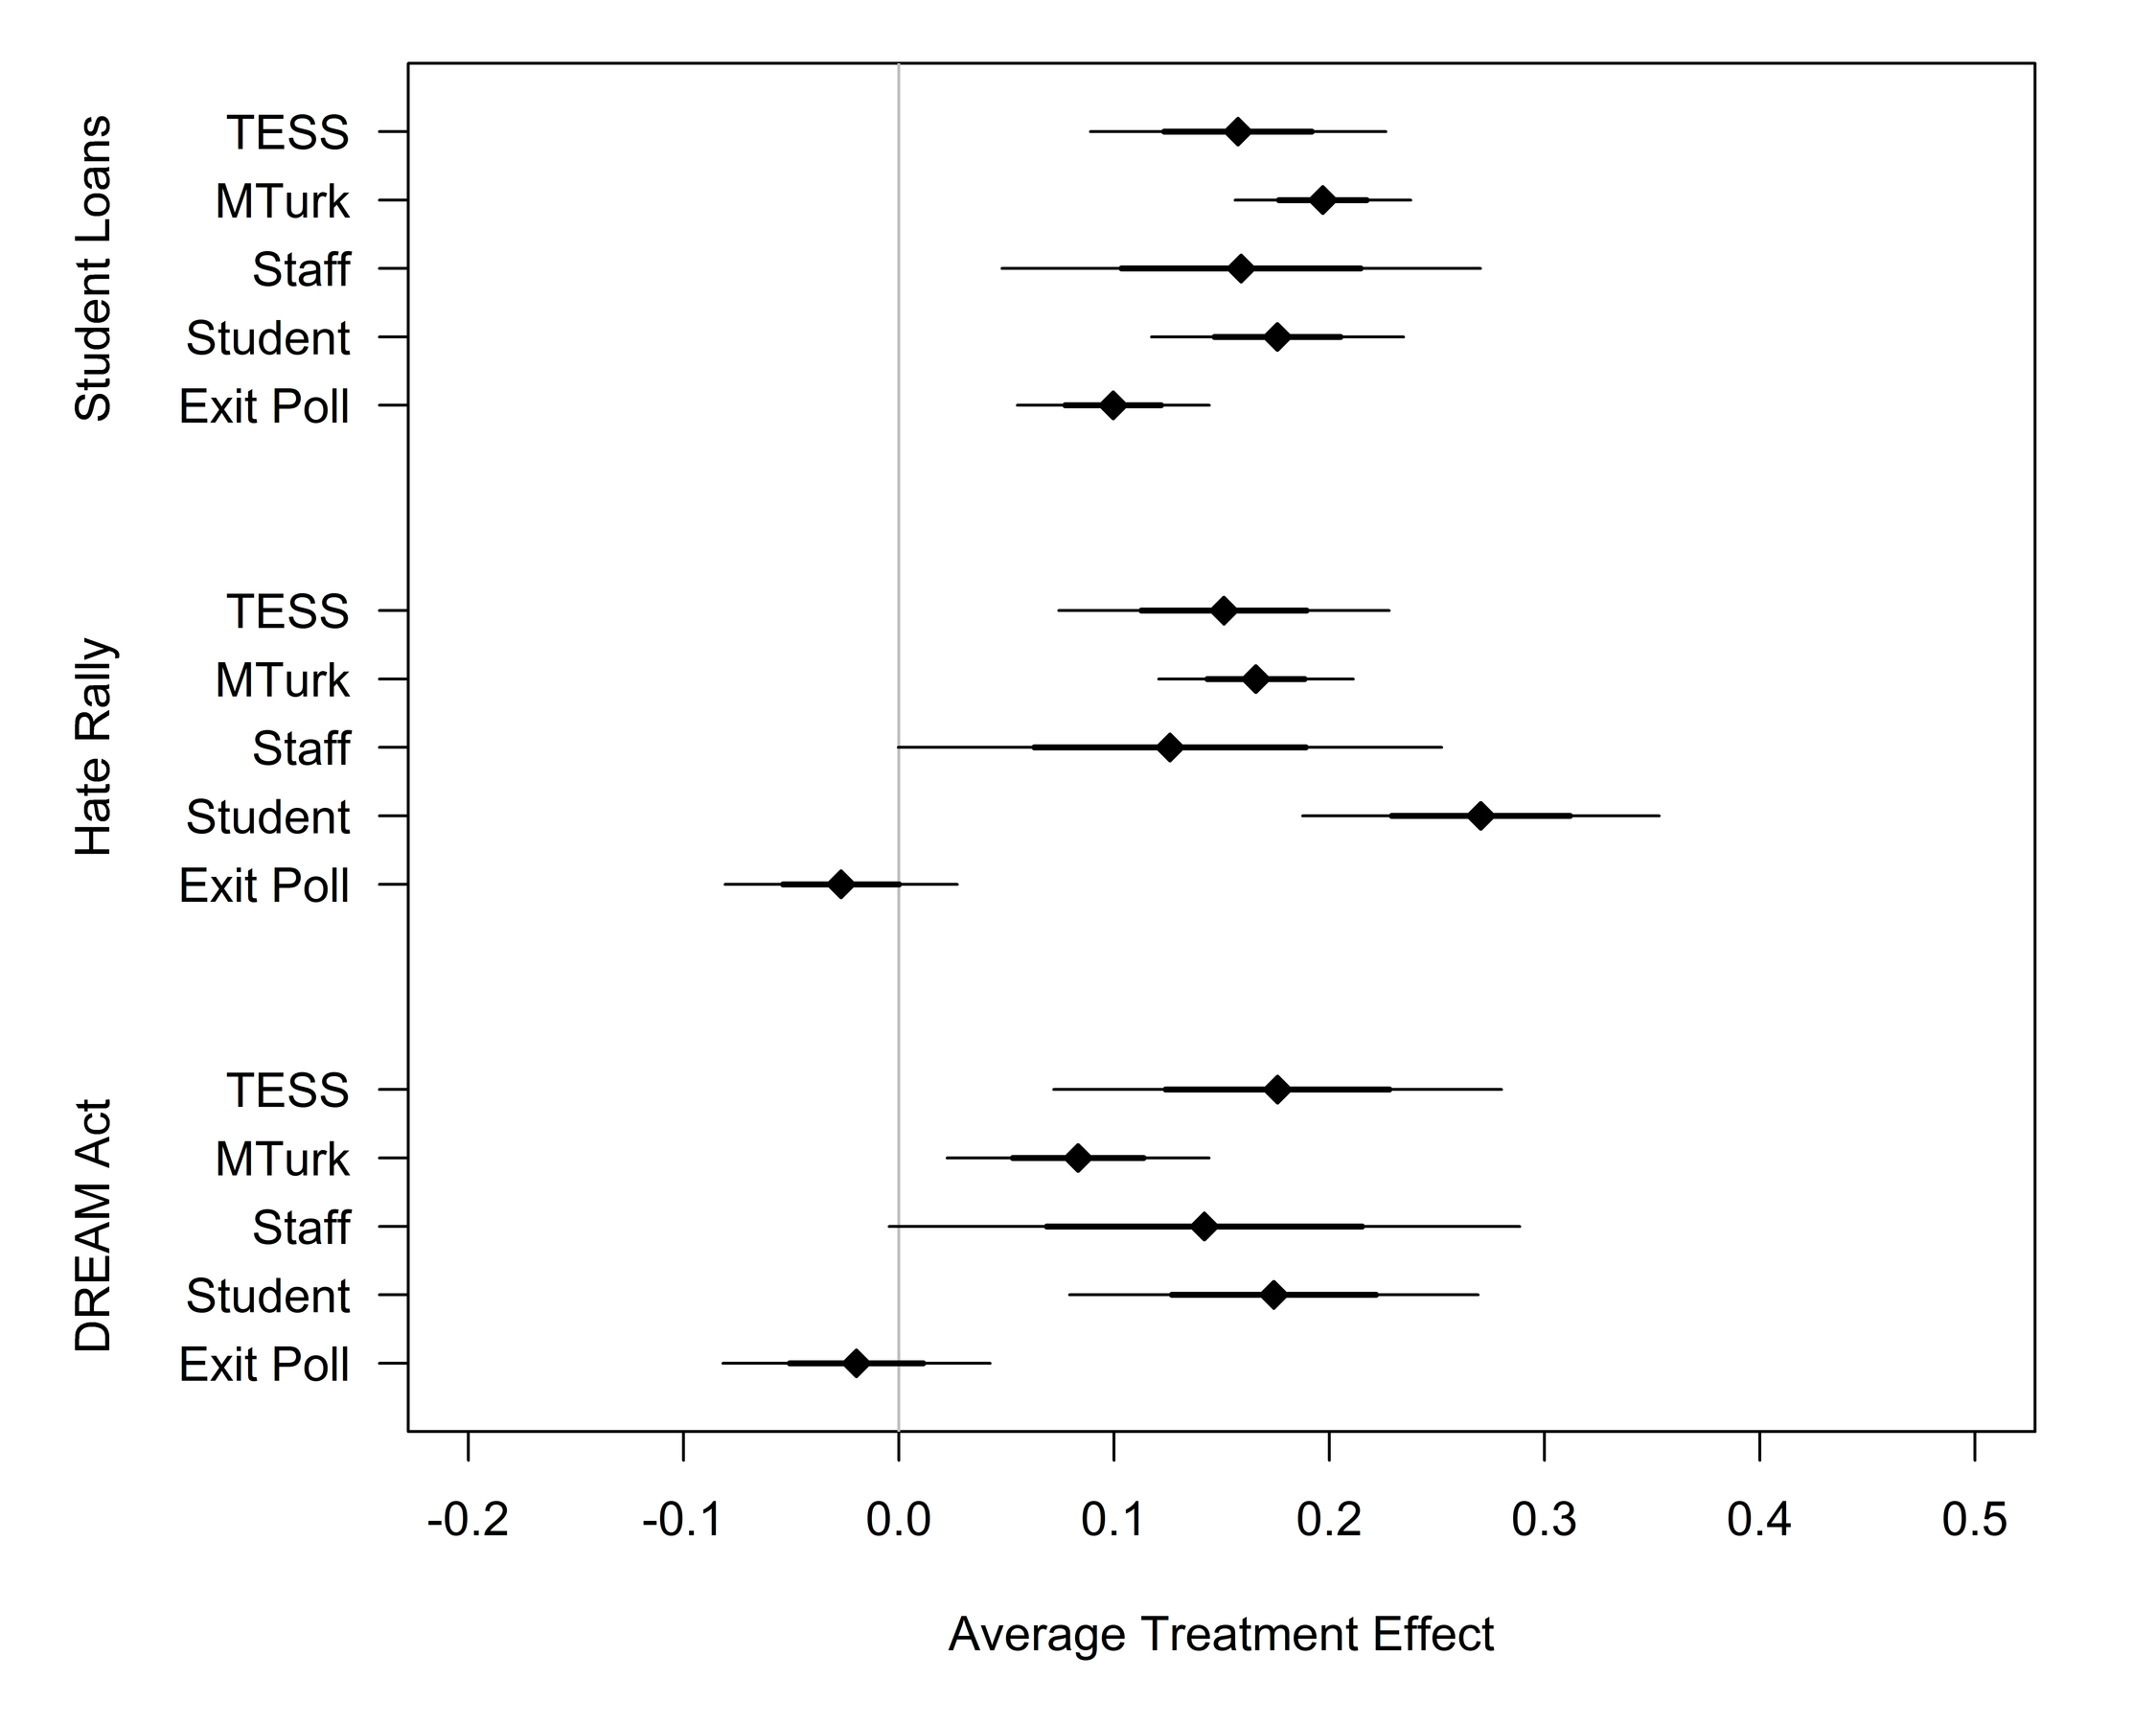
\includegraphics[height=.95\textheight]{images/mullinix3}
\end{center}
}


\frame{
\begin{center}
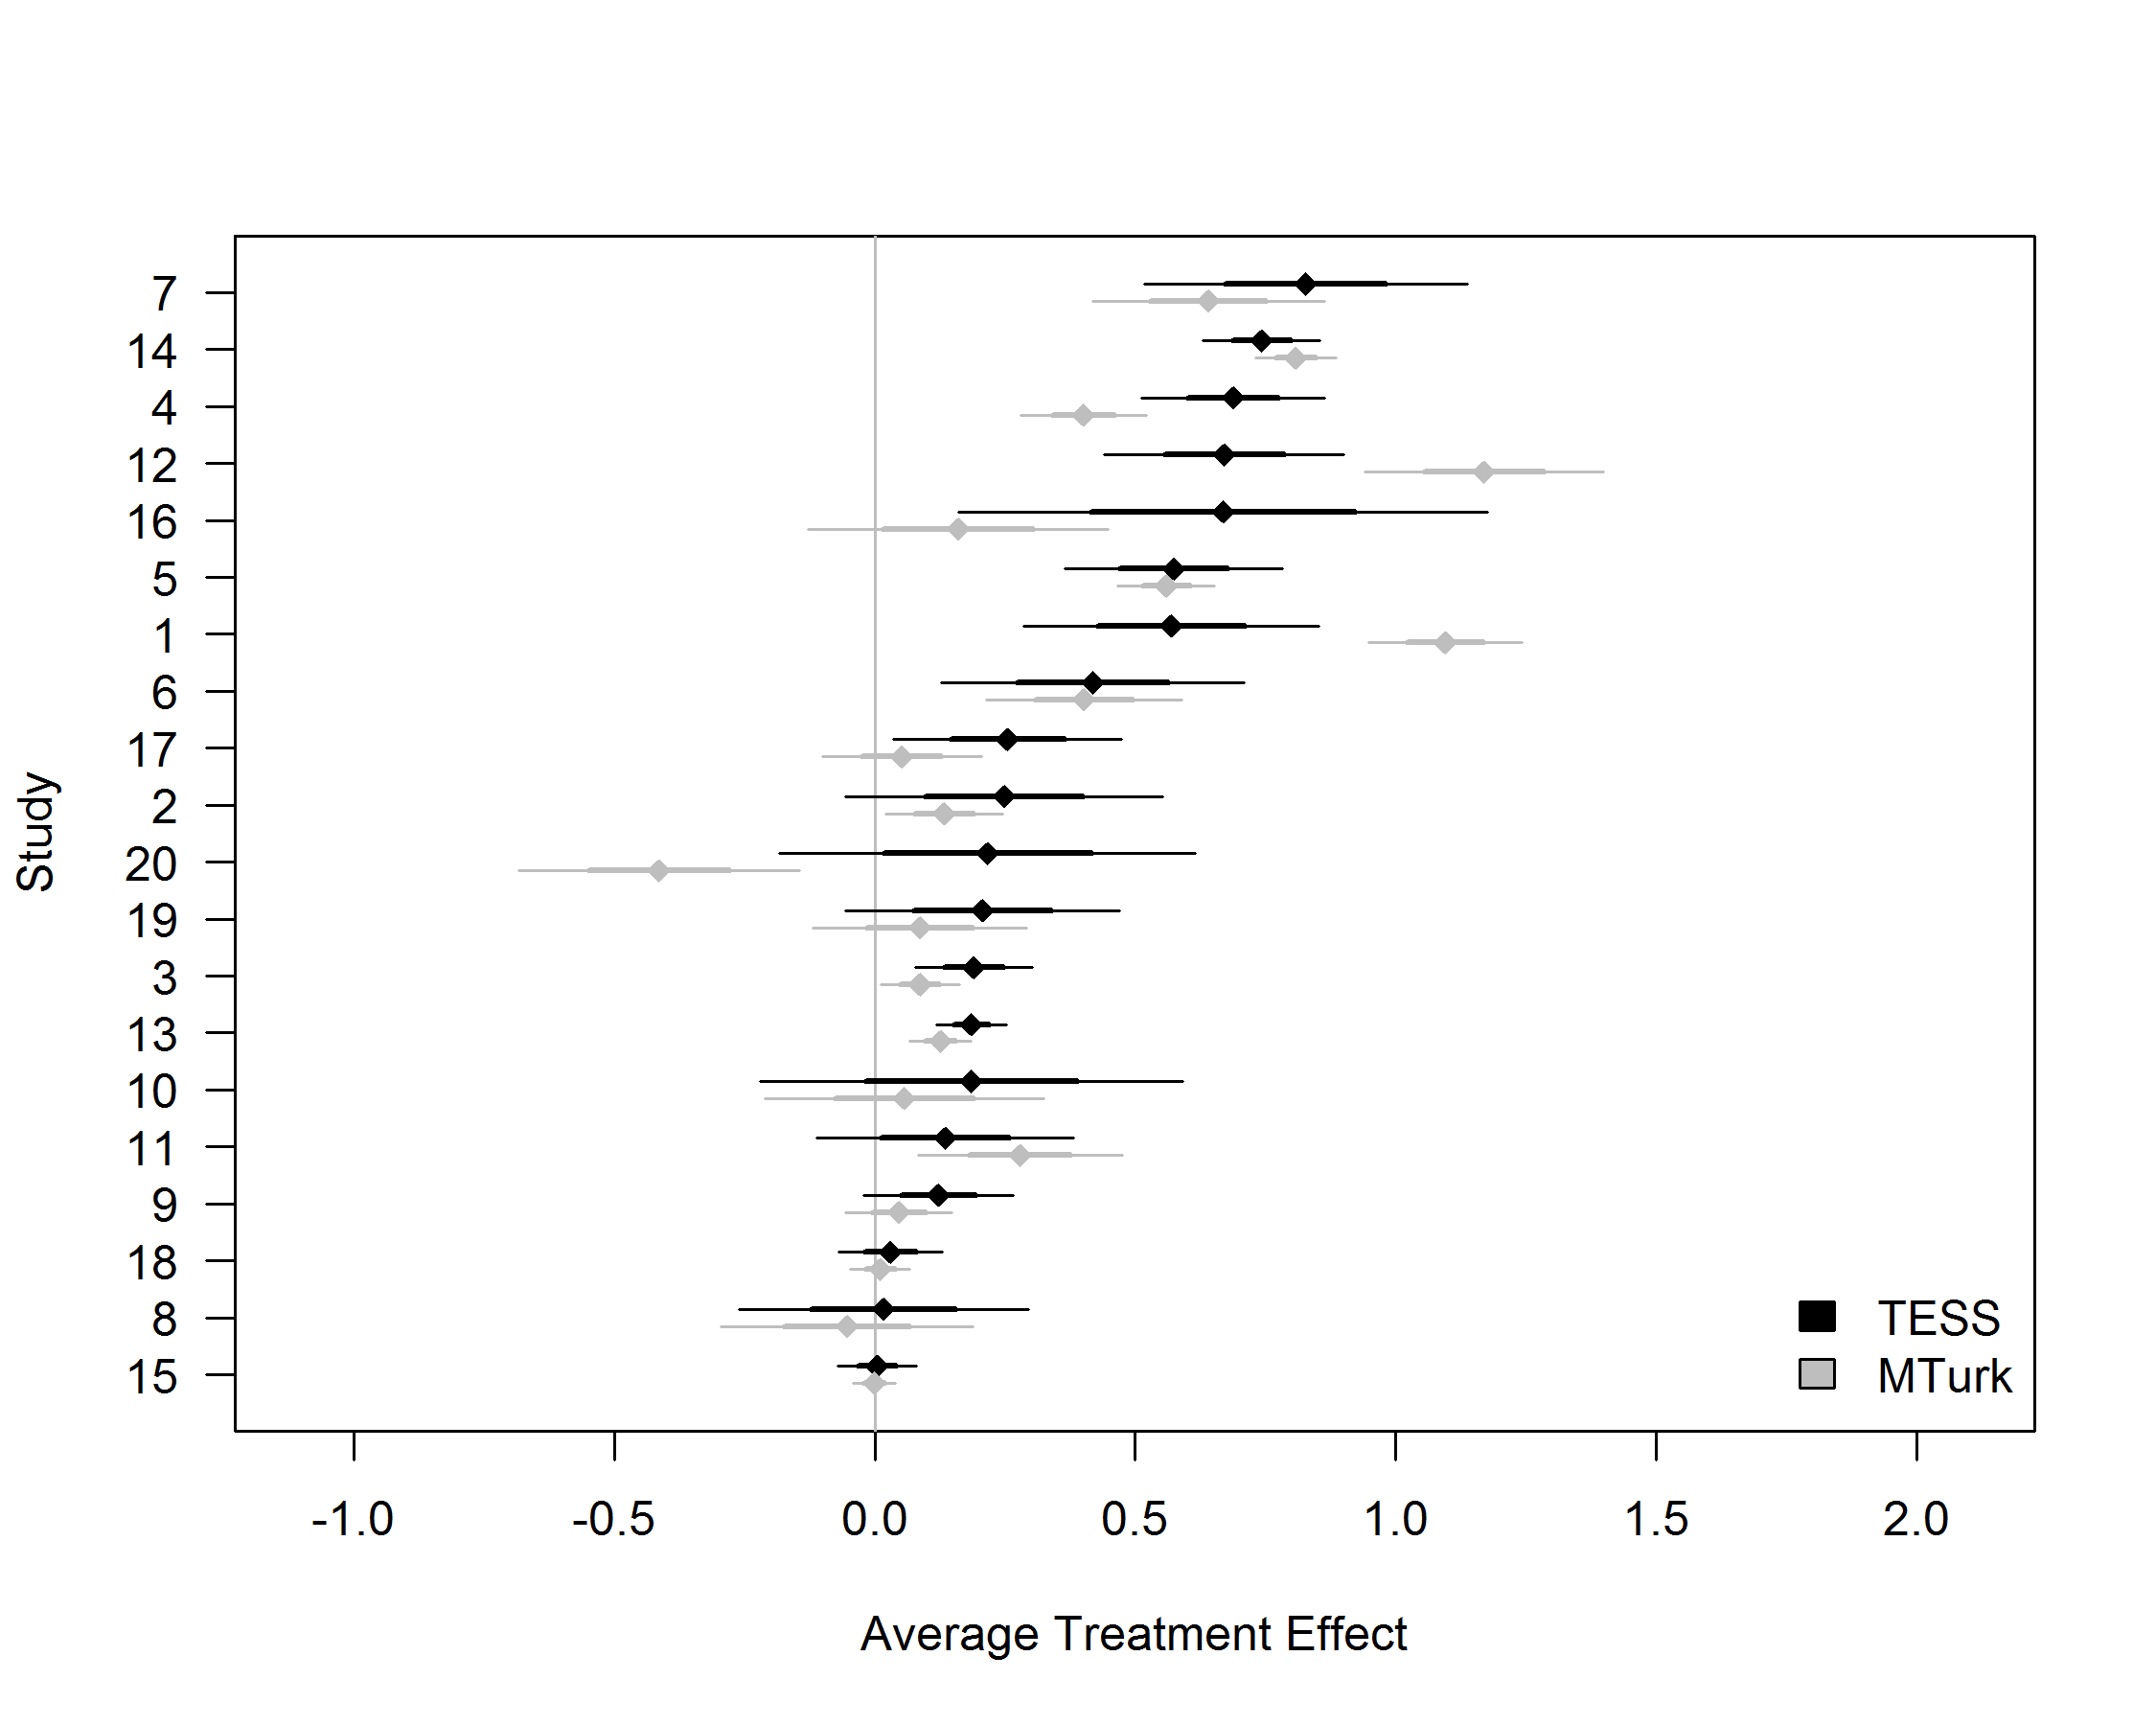
\includegraphics[width=1.1\textheight, trim=0in 0in 0in 0.5in, clip]{images/mullinix1}
\end{center}
}

\againframe<3-4>{myview}

\frame{
\frametitle{Common Differences}
\begin{itemize}\itemsep1em
\item Most common thing to focus on is demographic representativeness
	\begin{itemize}
	\item Sears (1986): ``students aren't real people''
	\item \href{http://www.slate.com/articles/health_and_science/science/2013/05/weird_psychology_social_science_researchers_rely_too_much_on_western_college.html}{Western, educated, industrialized, rich, democratic (WEIRD) psychology participants}
	\end{itemize}
\item<2-> But do those characteristics actually matter?
\end{itemize}
}

\frame{
\frametitle{Common differences}

Shadish, Cook, and Campbell tell us to think about:
	\begin{itemize}
	\item Surface similarities
	\item \textbf<2->{Ruling out irrelevancies}
	\item \textbf<2->{Making discriminations}
	\item Interpolation/extrapolation
	\end{itemize}
}


\frame{
\frametitle{{\normalsize Focus on effect heterogeneity}}

\begin{itemize}
\item<2-> \textbf{Constant effects}: $TE_i$ and $Y_{i0}$ are same for all observations
\item<3-> \textbf{Homogeneous effects}: $TE_i$ is same for all observations
\item<4-> \textbf{Heterogeneous effects}: $TE_i$ is different for all observations
\end{itemize}

}

\frame{
\frametitle{{\normalsize Focus on effect heterogeneity}}

\small

\begin{itemize}\itemsep0.5em
\item Think about and make an evidence-based argument for why you think there are (or are not) heterogeneous effects
\item<2-> If you think there is heterogeneity, then we probably do not care about the SATE anyway
\item<3-> Conditional Average Treatment Effect: $E[Y_{1i} | X = 1, Z=z] - E[Y_{0i} | X = 0, Z=z]$
\end{itemize}
}



\subsection{Model-based}
\frame{\tableofcontents[currentsection, currentsubsection, subsubsectionstyle=hide]}

\frame{

\frametitle{Stratification/Blocking}

\small

As soon as we care about heterogeneous effects, it makes sense to stratify and block on factors that might moderate the treatment effect.

\vspace{0.5em}

\onslide<2->{As soon as we identify all sources of heterogeneity, it doesn't matter what sample we use because effects are \textit{by definition} homogeneous within such strata.}

\vspace{0.5em}

\onslide<3->{But, we never know when we've reached that point!}

}



\frame{

If we acknowledge and start thinking about effect heterogeneity, does this mean we can use any convenient group of participants as if they were probability samples?

\vspace{1em}

No. Of course not.
}


% defining your convenience sample
\frame{
	\frametitle{{\normalsize Not All ``Samples'' Are Alike}}
	
	\small
	\begin{itemize}\itemsep0.25em
		\item<1-> Different types:
			\begin{itemize}
				\item<2-> Passive/opt-in/``river sampling''
				\item<3-> Sample of convenience
					\begin{itemize}
					\item Snowball sample
					\item Students
					\item Crowdsourcing
					\end{itemize}
			\end{itemize}
		\item<4-> Differ in numerous ways
			\begin{itemize}
			\item Cost
			\item ``Experience''
			\item Attentiveness
			\item Demographics
			\end{itemize}
	\end{itemize}
}

\frame{
\frametitle{Costs per participant}

From one of my studies:\\

\vspace{1em}

\centering
\begin{tabular}{l r r r}
Sample	& Cost	& n	& Cost/participant\\ \midrule
National	& \$13200	& 593	& \$22.26\\
Exit Poll	& \$3000	& 741	& \$4.05\\
Students	& \$0	& 299	& \$0\\
Staff		& \$1280	& 128	& \$10.00\\
MTurk	& \$550	& 1024	& \$0.54\\
Ads		& \$636	& 80		& \$7.95\\
\bottomrule
\end{tabular}
}

\frame{
\frametitle{Participant Experience}

\small

\begin{itemize}\itemsep0.5em
\item A lot of growing concern about experience
\item Larger literature on ``panel conditioning''
	\begin{itemize}
	\item Inconclusive evidence
	\end{itemize}
\item<3-> Some numbers:
	\begin{itemize}
	\item<3-> MTurk workers are doing 100+ studies per month
	\item<4-> Numbers are the same for YouGov panelists
	\end{itemize}
\end{itemize}

}


\frame{}

% reweighting; pscore methods
\frame{
\frametitle{Reweighting}
\begin{itemize}\itemsep0.5em
\item If effects are heterogeneous, it may be possible to \textit{reweight} unrepresentative data to match a population
\item Any method for this is ``model-based'' (rather than ``design-based'')
\item Not widely used or evaluated (yet)
\item All techniques build on the idea of stratification
\end{itemize}
}


\frame{
	\frametitle{Review of Stratification}
	
	\small
	\begin{enumerate}\itemsep0.25em
		\item Define population
		\item Construct a sampling frame
		\item Identify variables we already know about units in the sampling frame
		\item Stratify sampling frame based on these characteristics
		\item Collect an SRS within each stratum
		\item Aggregate our results
	\end{enumerate}
}


\frame{
	\frametitle{Post-Stratification}
	\begin{itemize}\itemsep0.5em
		\item Used to correct for nonresponse, coverage errors, and sampling errors
		\item<2-> Reweight sample data to match population distributions
			\begin{itemize}
				\item Divide sample and population into strata
				\item Weight units in each stratum so that the weighted sample stratum contains the same proportion of units as the population stratum does
			\end{itemize}
		\item<3-> There are numerous related techniques
	\end{itemize}
}

\frame{
	\frametitle{{\normalsize Post-Stratification: Example}}
	
	\normalsize
	\begin{itemize}\itemsep0.25em
		\item Imagine our sample ends up skewed on immigration status and gender relative to the population\\
	\end{itemize}
	\vspace{0.5em}
	{\small
	\begin{tabular}{lrrlr}
		\hline
		Group             & Pop. & Sample & Rep.                &              Weight \\ \hline
		Native-born, Female    &  .45 &     .5 & \onslide<2->{Over}  & \onslide<3->{0.900} \\
		Native-born, Male      &  .45 &     .4 & \onslide<2->{Under} & \onslide<4->{1.125} \\
		Immigrant, Female &  .05 &    .07 & \onslide<2->{Over}  & \onslide<4->{0.714} \\
		Immigrant, Male   &  .05 &    .03 & \onslide<2->{Under} & \onslide<4->{1.667}\\  \hline
	\end{tabular}
	}
	\begin{itemize}
	\item PS weight is just $w_{ps} = N_l / n_l$
	\end{itemize}
}


\frame{
	\frametitle{Post-Stratification}
	\begin{itemize}\itemsep1em
		\item This is the basis for inference in non-probability samples
		\begin{itemize}
			\item \textit{Demographic} representativeness
		\end{itemize}
		\item Online panels will reweight sample based on age, sex, education, etc.
		\item Purely design-based surveys are increasingly rare
	\end{itemize}
}


\frame{
\frametitle{The Xbox Study}

\begin{center}
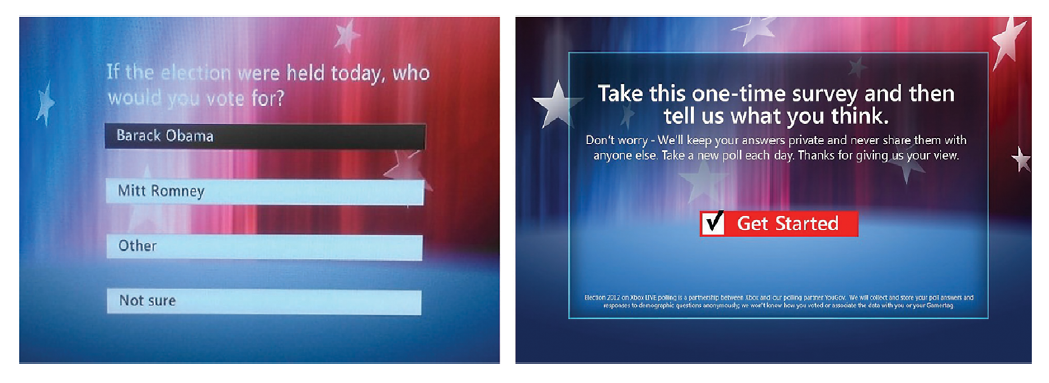
\includegraphics[width=\textwidth]{images/wangetal2}
\end{center}

{\footnotesize Wang et al. 2015. ``Forecasting elections with non-representative polls.'' \textit{International Journal of Forecasting}.\par}

}


\frame{
\frametitle{The Xbox Study}

\begin{center}
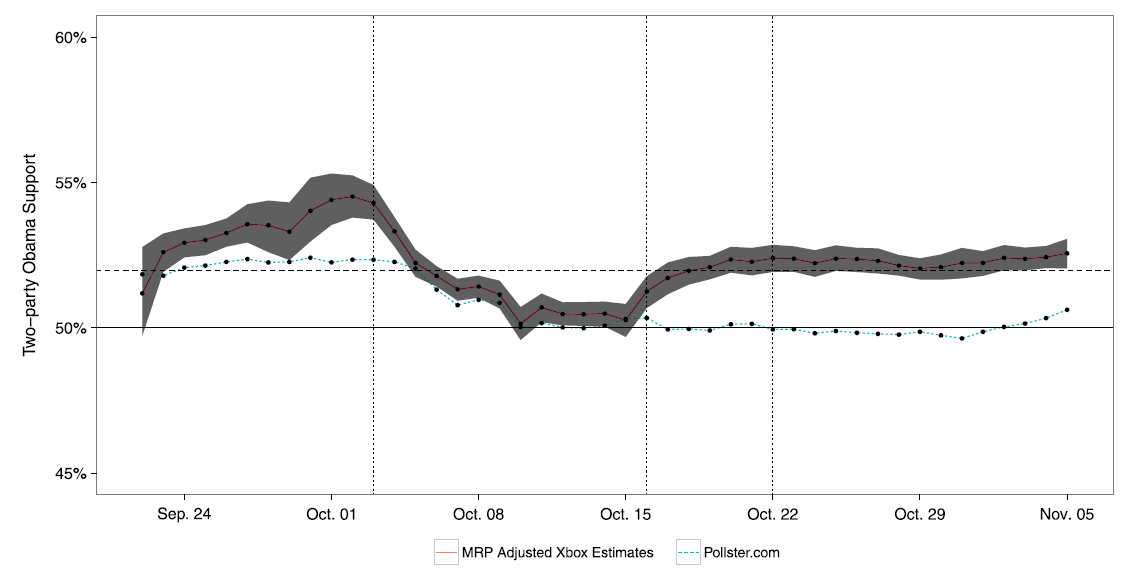
\includegraphics[width=\textwidth]{images/wangetal1}
\end{center}

{\footnotesize Wang et al. 2015. ``Forecasting elections with non-representative polls.'' \textit{International Journal of Forecasting}.\par}

}



\frame{

\vspace{-1.5em}
\begin{center}
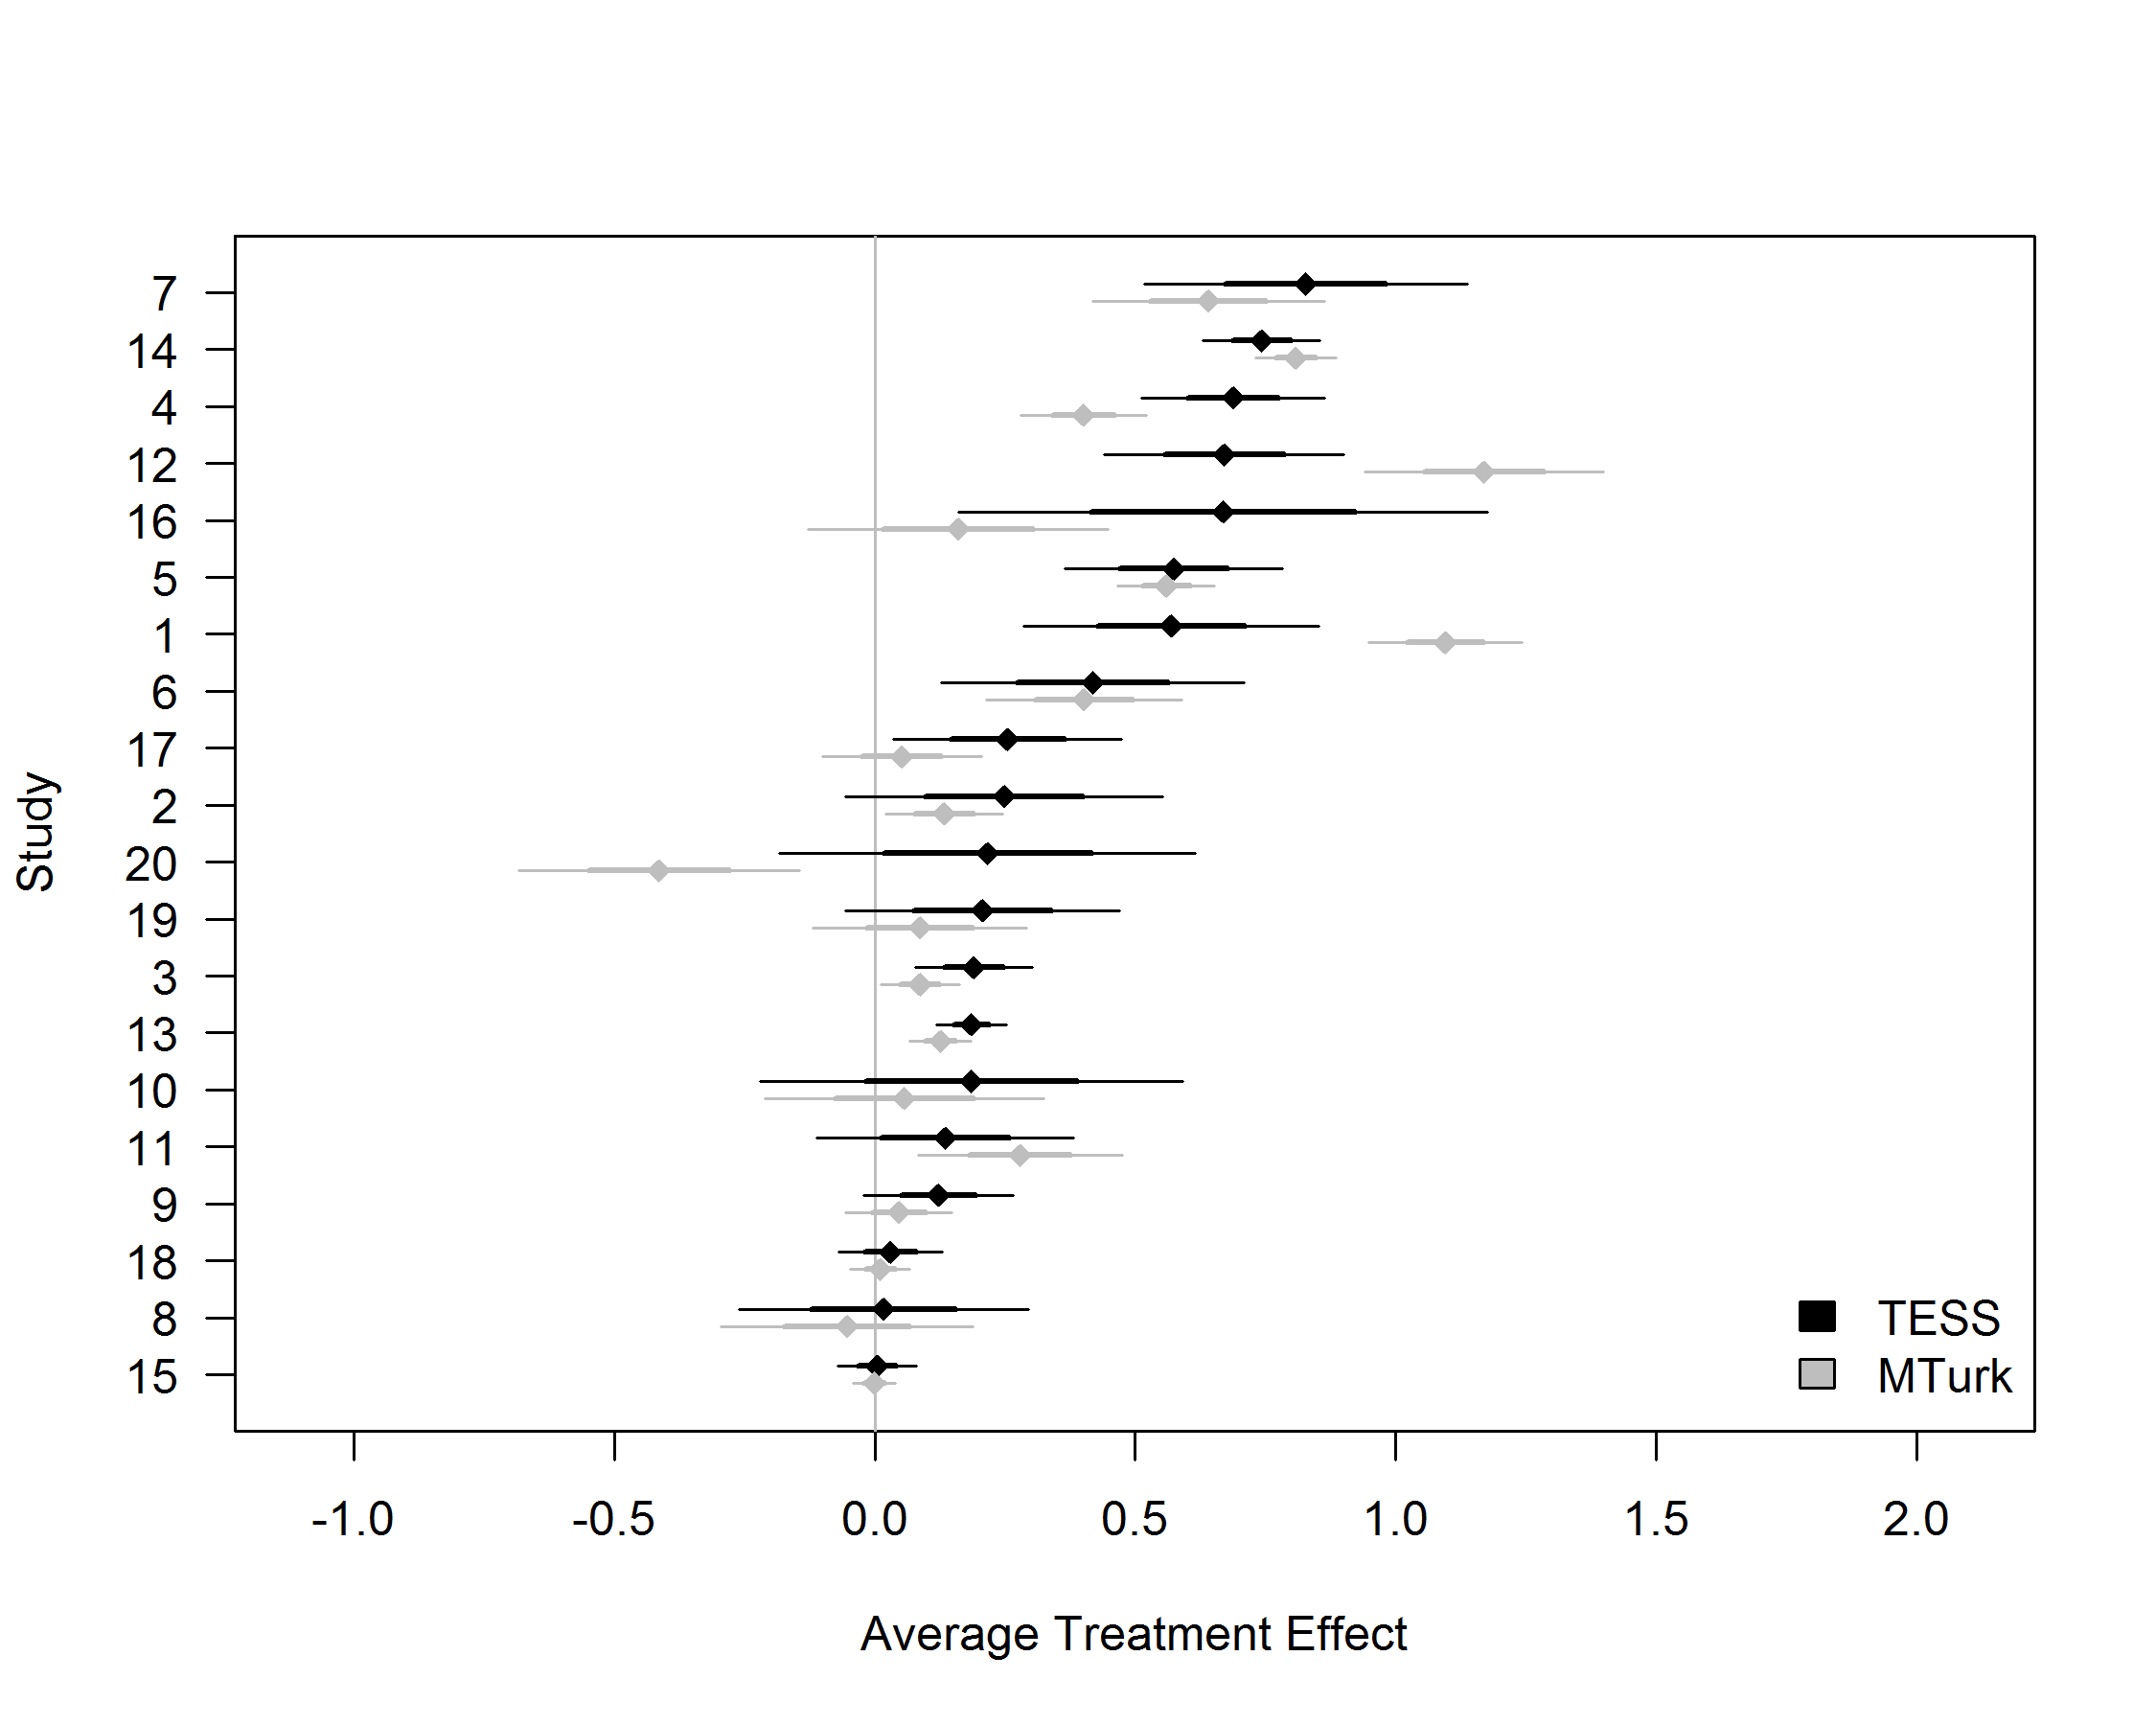
\includegraphics[width=.85\textwidth]{images/mullinix1}
\end{center}
{\footnotesize Mullinix et al. 2015. ``The Generalizability of Survey Experiments.'' \textit{Journal of Experimental Political Science}.\par}
}

\frame{
\vspace{-1em}
\begin{center}
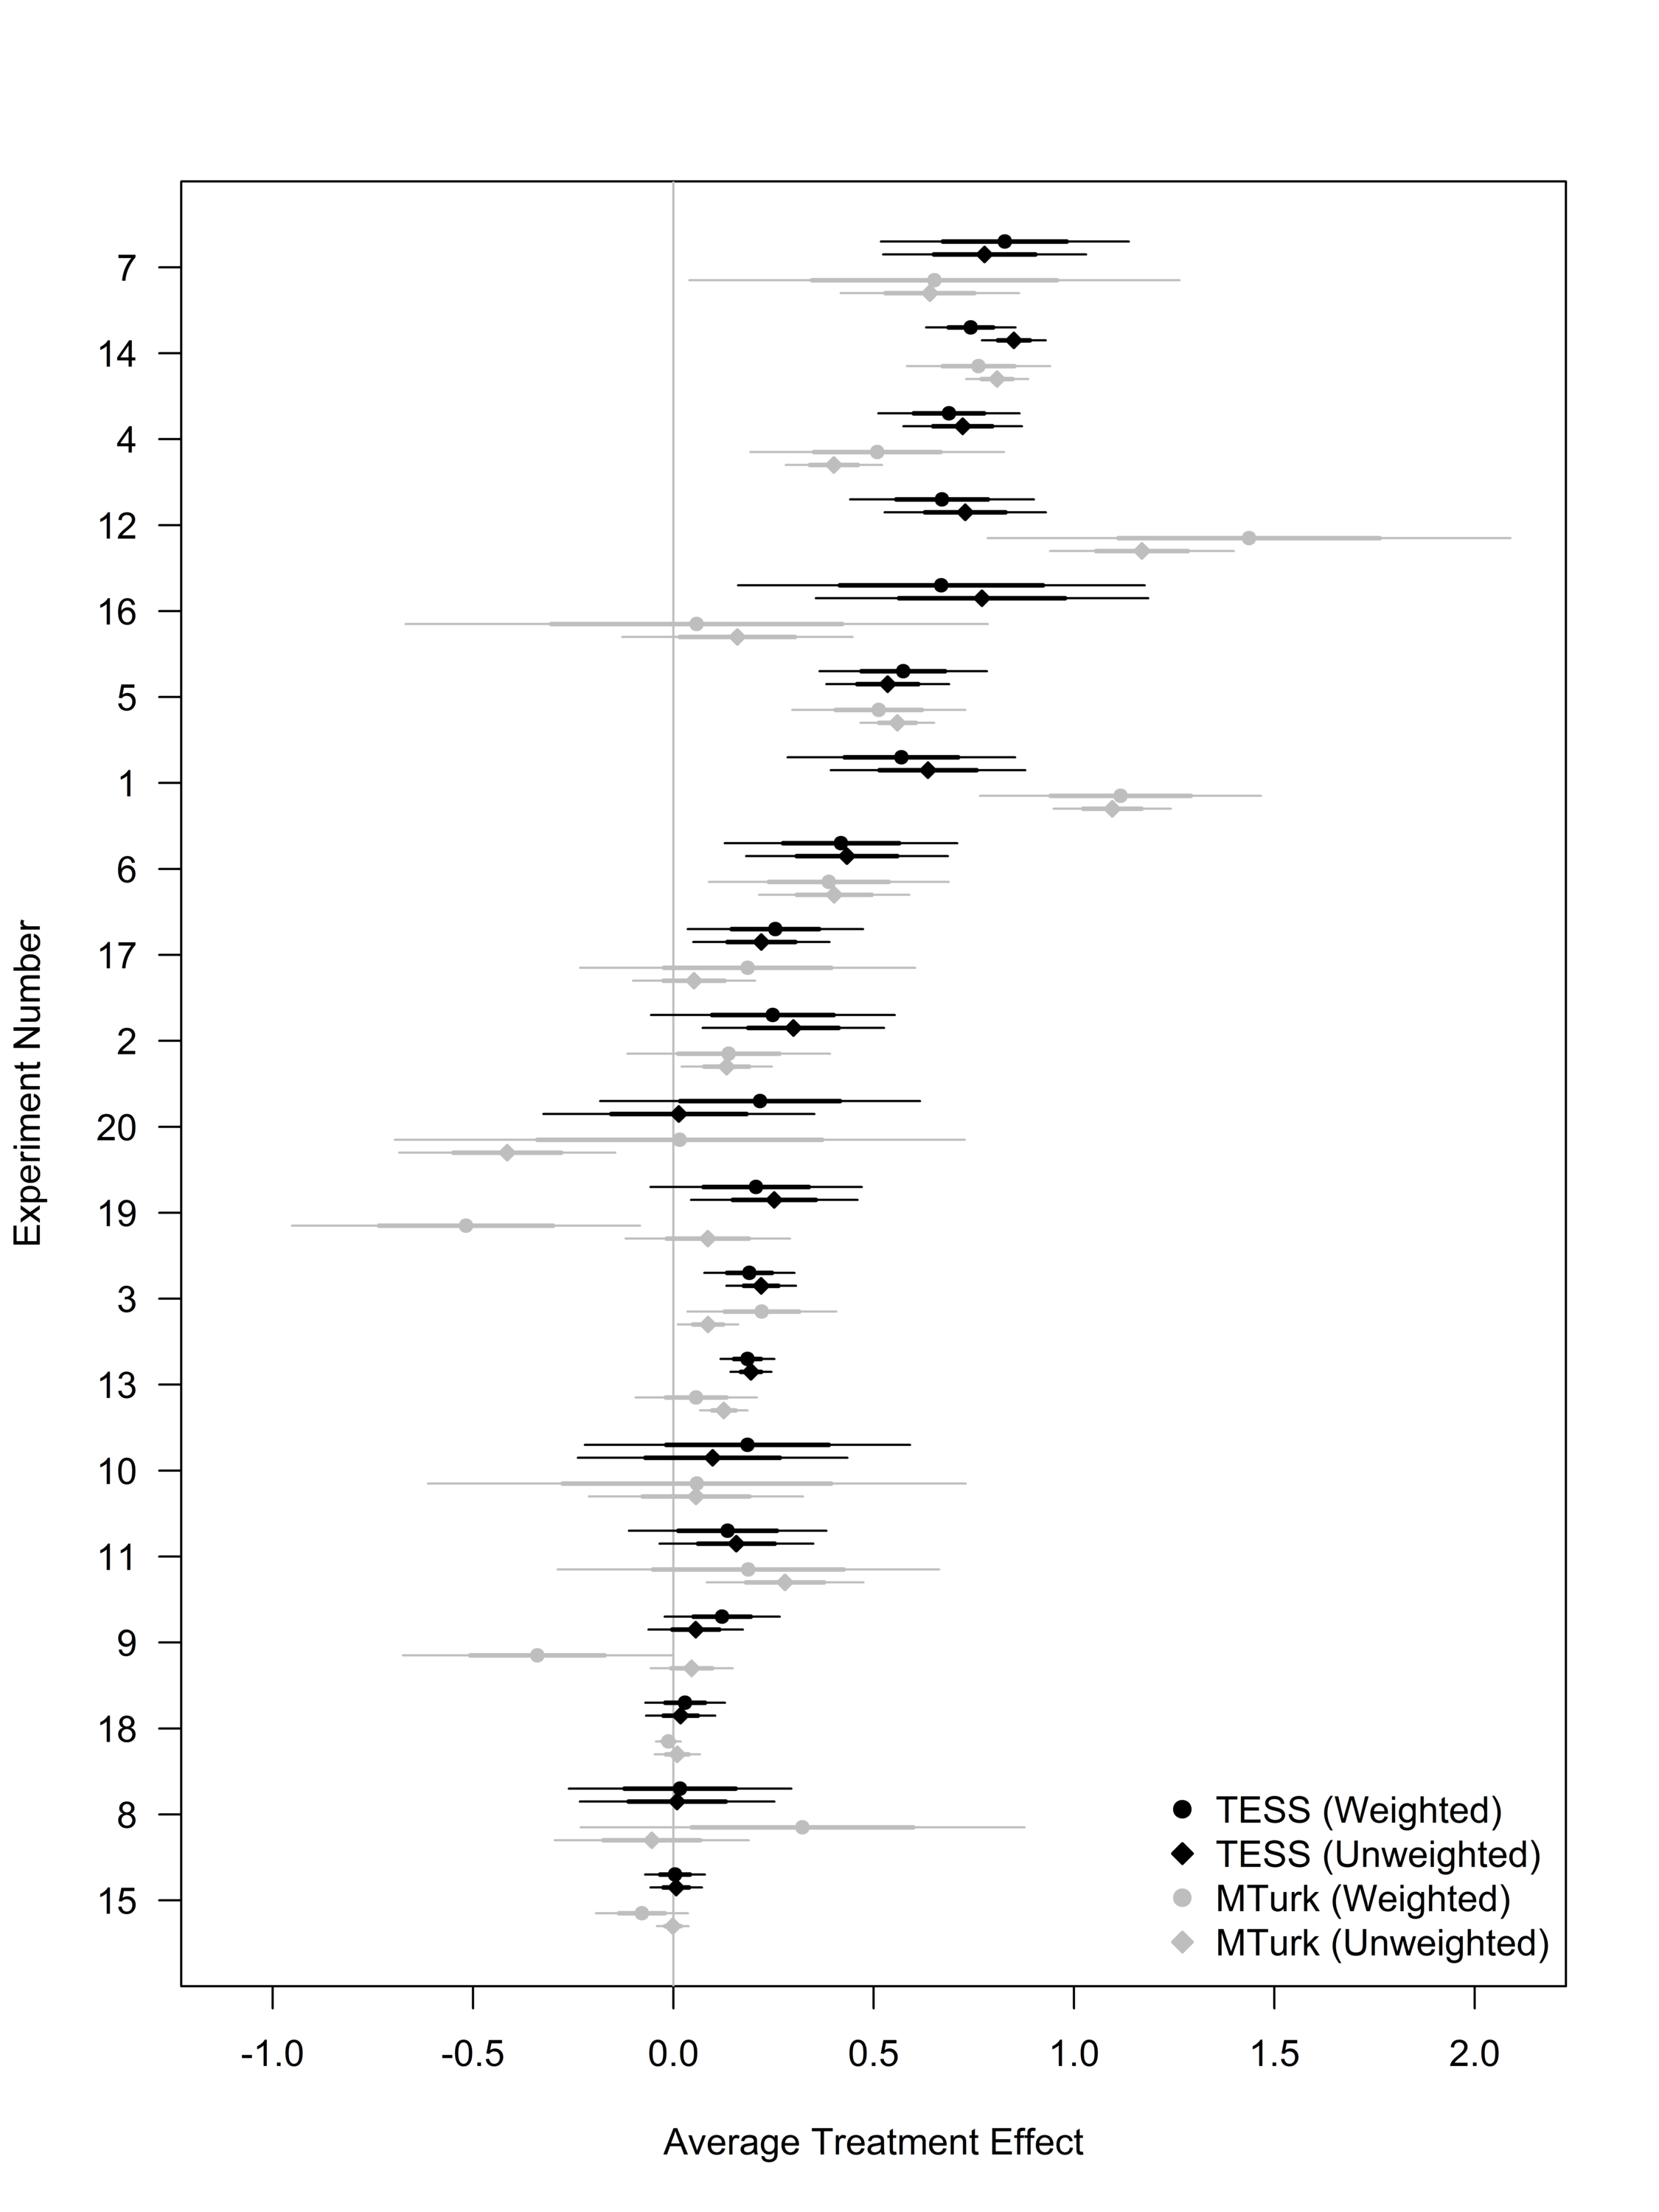
\includegraphics[width=.8\textheight]{images/mullinix2}
\end{center}
}



\frame{
\frametitle{{\normalsize Propensity Score Approach}}

\small

\begin{enumerate}\itemsep-0.2em
\item Define a target population 
\item Estimate a propensity score model
	\begin{itemize}\footnotesize
	\item Pool experimental samples and target population units
	\item Predict membership of all target and sample units in the experimental sample
	\end{itemize}
\item Using fitted logits, divide population \& sample into strata
\item Estimate stratum-specific ATE
\item Calculate weighted average of stratum-level estimates
\end{enumerate}
}


\frame{
\frametitle{{\normalsize Propensity Score Approach}}

Target population average treatment effect:
\begin{equation}
\sum_{v=1}^{5} p(v)T(v)
\end{equation}
where $p(v)$ is the proportion of the target population in a given stratum, $v$, and $T(v)$ is the estimated effect from stratum $v$ of the experimental sample
}


\frame{
\frametitle{Propensity Score Approach}

Effect variance:
\begin{equation}
\sum_{v=1}^{5} p(v)^2 V(v),
\end{equation}
where $V(v)$ is the variance of the estimated experimental sample effect for stratum $v$
}



\frame{
\frametitle{Propensity Score Subclassification Estimator}
\begin{columns}
\column{\dimexpr\paperwidth-12pt}
\scriptsize
\begin{tabular}{rrrrrrrrr} \toprule
& \multicolumn{2}{c}{Weights} & \multicolumn{6}{c}{Estimates}\\
Stratum & Nat'l & Sample & Loan & DREAM 1 & DREAM 2 & Rally \\% & Rally (Distant) & Rally (Local) \\ 
  \midrule
  1 & 0.20 & 0.83 & 0.94 (0.08) & 0.06 (0.11) & -0.22 (0.12) & 0.74 (0.10) \\% & 0.77 (0.15) & 0.72 (0.15) \\ 
  2 & 0.20 & 0.11 & 0.99 (0.26) & 0.22 (0.37) & -0.28 (0.36) & 0.77 (0.29) \\% & 0.85 (0.39) & 0.70 (0.42) \\ 
  3 & 0.20 & 0.04 & 1.28 (0.43) & -0.61 (0.58) & -1.76 (0.54) & 1.00 (0.45) \\% & 0.75 (0.64) & 1.26 (0.64) \\ 
  4 & 0.20 & 0.01 & 1.99 (0.73) & 0.29 (1.12) & 0.56 (0.89) & 1.44 (0.79) \\% & 3.13 (1.95) & 1.54 (0.63) \\ 
  5 & 0.20 & 0.00 &  &  &  &  &  &  \\ \midrule
  Sample & - & - & 1.04 (0.30) & -0.01 (0.44) & -0.34 (0.38) & 0.79 (0.33) \\% & 1.05 (0.60) & 0.86 (0.37) \\ 
  Nat'l & - & - & 1.14 (0.18) & 0.02 (0.22) & -0.94 (0.23) & 0.94 (0.19) \\% & 1.01 (0.26) & 0.93 (0.27) \\ 
   \bottomrule
\end{tabular}
\end{columns}
}


\frame{
\frametitle{{\normalsize So does reweighting solve everything forever?}}

\begin{itemize}\itemsep0.25em
\item<2-> Need well-defined target population
	\begin{itemize}
	\item and detailed covariate data
	\item and large stratum sizes
	\end{itemize}
\item<3-> Purely model-based, so only as good as the model
	\begin{itemize}
	\item What unobservables might there be?
	\item What reweighting might worse bias?
	\end{itemize}
\item<4-> Non-coverage is a potential problem
\item<5-> Not well-tested on experimental data
\end{itemize}

}



\questions

\section[SUTO]{Other Notions of External Validity}
\frame{\tableofcontents[currentsection,subsubsectionstyle=hide]}


\frame{
\frametitle{SUTO Framework}
\begin{itemize}\itemsep0.5em
\item Cronbach (1986) talks about generalizability in terms of UTO
\item Shadish, Cook, and Campbell (2001) speak similarly of:
	\begin{itemize}
	\item \textbf{S}ettings
	\item \textbf{U}nits
	\item \textbf{T}reatments
	\item \textbf{O}utcomes
	\end{itemize}
\item External validity depends on all of these
\end{itemize}
}


\frame{
\begin{columns}[t]
\begin{column}{0.5\textwidth}
	\begin{block}{Population}
		\begin{itemize}
		\item Setting
		\item Units
		\item Treatments
		\item Outcomes
		\end{itemize}
	\end{block}
\end{column}
\begin{column}{0.5\textwidth}
	\begin{block}{Your Study}
		\begin{itemize}
		\item Setting
		\item Units
		\item Treatments
		\item Outcomes
		\end{itemize}
	\end{block}
\end{column}
\end{columns}

\vspace{0.5em}

\small

\only<2->{In your study, how do these correspond?\\}
\only<3->{\hspace{5.7em} how do these differ?\\}
\only<4->{\hspace{5.7em} do these differences matter?\\}

}


\subsection[S]{Settings}

\frame{

\frametitle{Heterogeneity due to \textit{S}ettings}

\begin{itemize}\itemsep1em
\item We should expect heterogeneity related to settings!
\item How do we use/explore this?
	\begin{itemize}
	\item<2-> Comparative research designs where experiments provide measures for each case
	\item<3-> Over-time replications of the same design
	\item<4-> Replication of a design across contexts with unknown sources of variability?
	\end{itemize}
\item<5-> Can we control for context?
\end{itemize}

}


\frame{

\frametitle{Pretreatment Dynamics}

``If the experiment explores a communication that regularly occurs in `reality,' then reactions in the experiment might be contaminated by those `regular' occurrences prior to the experiment.'' \footnote{p.875 from Druckman \& Leeper. 2012. ``Learning More from Political Communication Experiments: Pretreatment and Its Effects.'' \textit{American Journal of Political Science} 56(4): 875--896.}

}

\frame{

\frametitle{Pretreatment Dynamics}

\small
\begin{itemize}
\item Pretreatment is a feature of an experimental setting, treatment, and sample, wherein the effect of the treatment has already occurred\footnote{Or, units having already been treated are otherwise affected differently.}
\item<2-> Consequences:
	\begin{itemize}\footnotesize
	\item Biased effect estimates
	\end{itemize}
\item<3-> Mitigation:
	\begin{itemize}\footnotesize
	\item Measure pretreatment
	\item Avoid ``pretreated'' treatments or contexts
	\item Study units not already treated
	\item Theorize repeated effects
	\end{itemize}
\end{itemize}

}

\frame{}







\questions






\subsection[U]{Unit}


\frame{

\frametitle{Heterogeneity due to \textit{U}nits}

Most commonly studied source of heterogeneity is covariate-related (i.e., characteristics of units).\\

\vspace{1em}

If we think there might be covariate-related effect heterogeneity, what can we do?

\begin{itemize}
\item Best solution: manipulate the moderator
\item Next best: block on the moderator
\item Least best: post-hoc exploratory approaches
\end{itemize}
}

\subsubsection{Blocking/Block Randomization}

\frame{

\frametitle{Block Randomization}

\small

\begin{itemize}\itemsep0.5em
\item<2-> Basic idea: randomization occurs within strata defined before treatment assignment
\item<3-> CATE is estimate for each stratum; aggregated to SATE
\item<4-> But\dots
	\begin{itemize}
	\item Blocked randomization only works in exactly the same situations where stratified sampling works
	\item Need to observe covariates pre-treatment in order to block on them, so works in panels but not cross-sectional designs
	\item More precise SATE estimate
	\end{itemize}
\end{itemize}

}



\questions

\subsubsection{Post-hoc Approaches}

\frame{
\frametitle{{\large Three Post-hoc Approaches}}

\begin{itemize}\itemsep0.5em
\item Suggestive evidence
\item Regression using treatment-by-covariate interactions
\item Automated approaches
\item<2-> (Replication and meta-analysis)
\end{itemize}

}



\frame{

\frametitle{Suggestive Evidence}

We can never know $Var(TE_i)$! \onslide<2->{But\dots}

\begin{itemize}\itemsep0.5em
\item<2-> Quantile-quantile plots
	\begin{itemize}
	\item<3-> Compare the distribution of $Y_0$'s to distribution of $Y_1$'s
	\item<3-> If homogeneity, a vertical shift in $Y_1$'s
	\item<3-> If heterogeneity, a slope $\neq$ 1
	\end{itemize}
\item<2-> Equality of variance tests
	\begin{itemize}
	\item<4-> If homogeneity, variance should be equal
	\item<4-> If heterogeneity, variances should differ
	\end{itemize}
\end{itemize}

}

\begin{frame}[fragile]

\frametitle{QQ Plots}

{\scriptsize
\begin{verbatim}
# y_0 data
set.seed(1)
n <- 200
y0 <- rnorm(n) + rnorm(n, 0.2)

# y_1 data (homogeneous effects)
y1a <- y0 + 2 + rnorm(n, 0.2)
# y_1 data (heterogeneous effects)
y1b <- y0 + rep(0:1, each = n/2) + rnorm(n, 0.2)

qqplot(y0, y1a, pch=19, xlim=c(-3,5), ylim=c(-3,5), asp=1)
curve((x), add = TRUE)
qqplot(y0, y1b, pch=19, xlim=c(-3,5), ylim=c(-3,5), asp=1)
curve((x), add = TRUE)
\end{verbatim}

}

\end{frame}


\frame{

\begin{center}
\only<1>{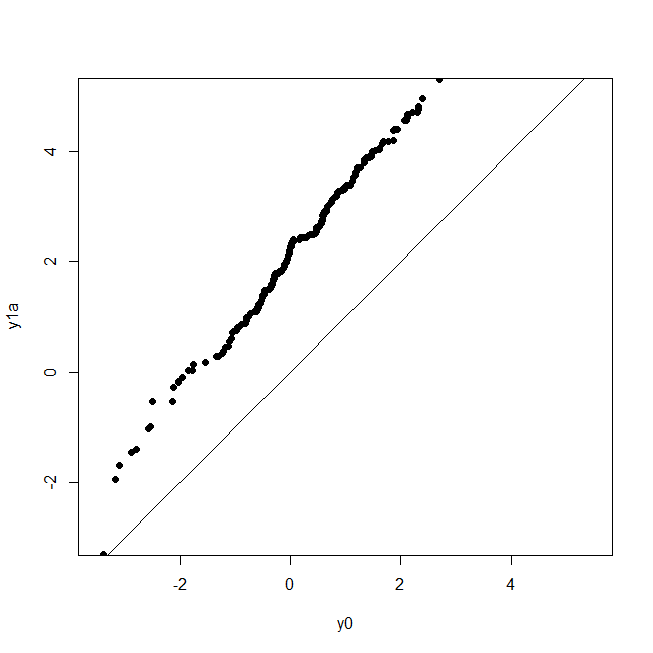
\includegraphics[height=\textheight]{images/qqplot1}}
\only<2>{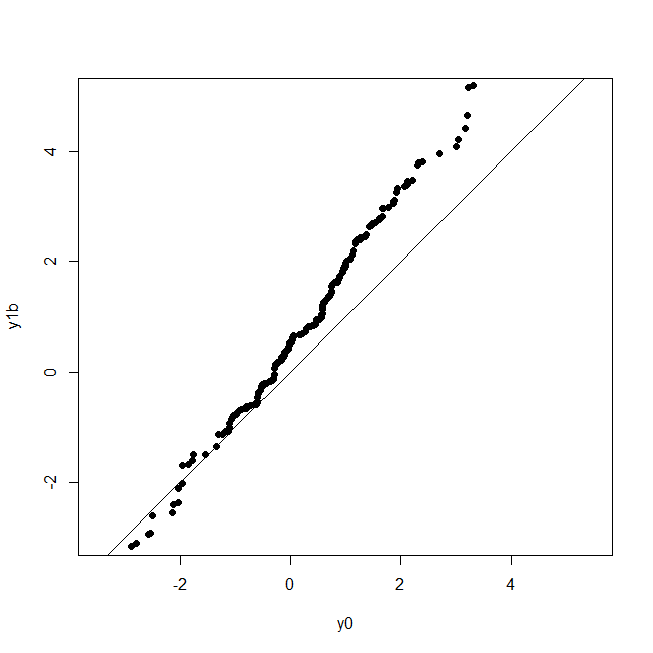
\includegraphics[height=\textheight]{images/qqplot2}}
\end{center}

}

\begin{frame}[fragile]

\frametitle{Equality of Variance tests}

\footnotesize

\begin{verbatim}
> var.test(y0, y1a)

        F test to compare two variances

data:  y0 and y1a
F = 0.60121, num df = 199, denom df = 199, 
  p-value = 0.0003635
alternative hypothesis: 
  true ratio of variances is not equal to 1
95 percent confidence interval:
 0.4549900 0.7944289
sample estimates:
ratio of variances 
         0.6012131 
\end{verbatim}

\end{frame}

\begin{frame}[fragile]

\frametitle{Equality of Variance tests}

\footnotesize

\begin{verbatim}
> var.test(y0, y1b)

        F test to compare two variances

data:  y0 and y1b
F = 0.53483, num df = 199, denom df = 199,
  p-value = 1.224e-05
alternative hypothesis:
  true ratio of variances is not equal to 1
95 percent confidence interval:
 0.4047531 0.7067133
sample estimates:
ratio of variances 
         0.5348312
\end{verbatim}

\end{frame}


\questions


\frame{\frametitle{Regression Estimation}}

\frame{

\frametitle{{\normalsize Aside: Regression Adjustment in Experiments, Generally}}

\begin{itemize}\itemsep0.5em
\item Recall the general advice that we do not need covariates in the regression to ``control'' for omitted variables (because there are none)
\item Including covariates can reduce variance of our SATE by explaining more of the variation in $Y$
\end{itemize}

}

\frame{

\frametitle{Scenario}

Imagine two regression models. Which is correct?

\begin{enumerate}
\item Mean-difference estimate of SATE is ``not significant''
\item Regression estimate of SATE, controlling for sex, age, and education, is ``significant''
\end{enumerate}

\onslide<2->{This is a small-sample dynamic, so make these decisions pre-analysis!}

}

\frame{

\frametitle{{\normalsize Treatment-Covariate Interactions}}

\normalsize

\begin{itemize}
\item The regression paradigm allows us to estimate CATEs using interaction terms
	\begin{itemize}
	\item $X$ is an indicator for treatment
	\item $M$ is an indicator for possible moderator
	\end{itemize}
\item<2-> SATE: $Y = \beta_0 + \beta_1 X + e$
\item<3-> CATEs: $$Y = \beta_0 + \beta_1 X + \beta_2 M + \beta_3 X*M + e$$
	\begin{itemize}
	\item<4-> Homogeneity: $\beta_3 = 0$
	\item<4-> Heterogeneity: $\beta_3 \neq 0$
	\end{itemize}

\end{itemize}

}



\frame{
\frametitle{BART}

\small
\begin{itemize}\itemsep0.5em
\item Estimate CATEs in a fully automated fashion
\item<2-> ``Bayesian Additive Regression Trees''
	\begin{itemize}
	\item Essentially an ensemble machine learning method
	\end{itemize}
\item<3-> Iteratively split a sample into more and more homogeneous groups until some threshold is reached using binary (cutpoint) decisions
\item<3-> Repeat this a bunch of times, aggregating across results
\end{itemize}
}

\frame{
\begin{center}
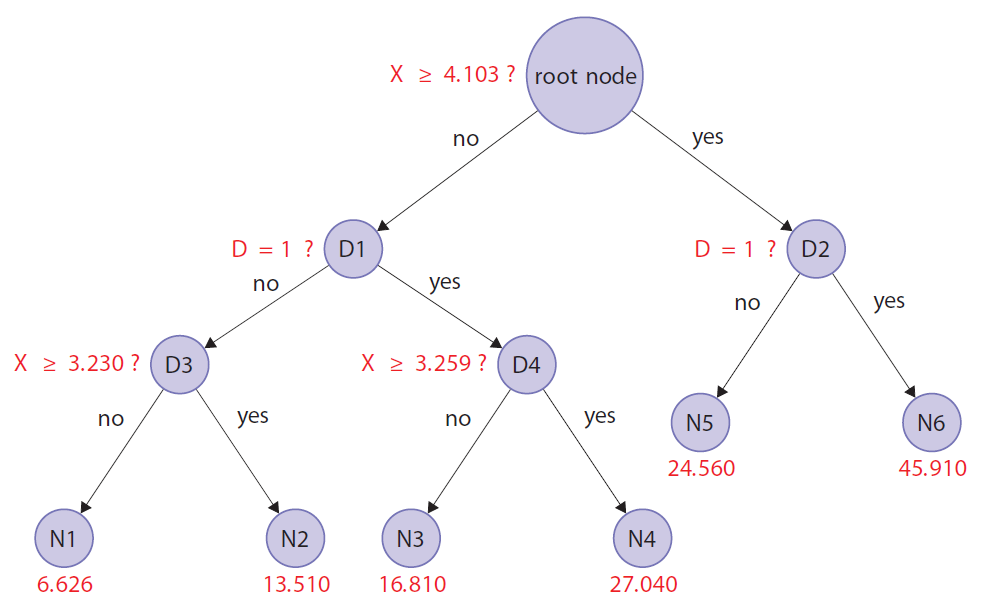
\includegraphics[width=\textwidth]{images/greenkern1}
\end{center}
{\footnotesize Green \& Kern. 2012. ``Modeling Heterogeneous Treatment Effects in Survey Experiments with Bayesian Additive Regression Trees.'' \textit{Public Opinion Quarterly} 76(3): 491--511.\par}
}

\frame{
\begin{center}
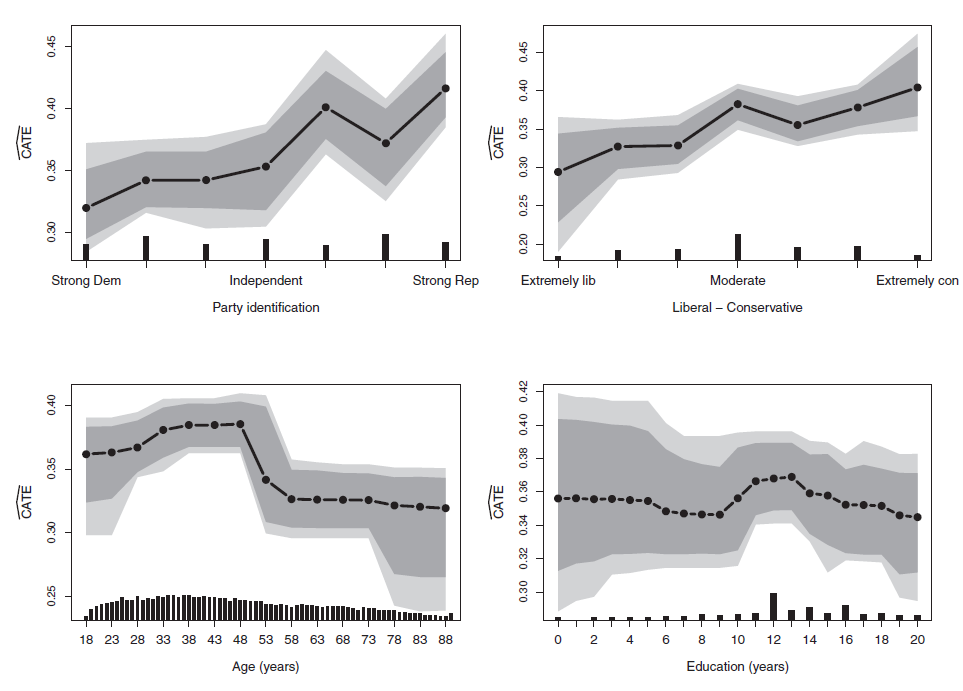
\includegraphics[height=.85\textheight]{images/greenkern2}
\end{center}
}


\frame{
\frametitle{Considerations}

\begin{itemize}\itemsep0.5em
\item BART is totally automated, conditional on the set of covariates used
\item Only really works with dichotomous covariates
\item Not widely used or tested
\item Totally post-hoc and atheoretical
\end{itemize}

}





\frame{

\frametitle{Considerations}

\small

\begin{itemize}
\item<2-> Coefficients on moderators have no causal interpretation without further conditioning on observables
\item<3-> Nearly unlimited potential moderators
	\begin{itemize}
	\item First-order interactions with every covariate in dataset
	\item Second-, third-order, etc. interactions
	\end{itemize}
\item<3-> Thus, multiple comparisons problem!
\item<4-> Power (esp. if $M$ is continuous)
\end{itemize}

}



\subsubsection{Manipulate the Moderator}


\frame{

Simply: Manipulating the moderator variable is the best way to estimate a heterogeneous effect!

\vspace{1em}

Why is this true?

}


\frame{

\frametitle{Complex Designs}

\small

\begin{itemize}
\item An experiment can have any number of conditions
	\begin{itemize}\footnotesize
	\item Up to the limits of sample size
	\item More than 8--10 conditions is typically unwieldy
	\end{itemize}
\item Typically analyze complex designs using ANOVA or regression, but we are still ultimately interested in pairwise comparisons to estimates SATEs
	\begin{itemize}\footnotesize
	\item Treatment--treatment, or treatment-control
	\item Without control group, we don't know which treatment(s) affected the outcome
	\end{itemize}
\end{itemize}

}


\begin{frame}
\begin{center}
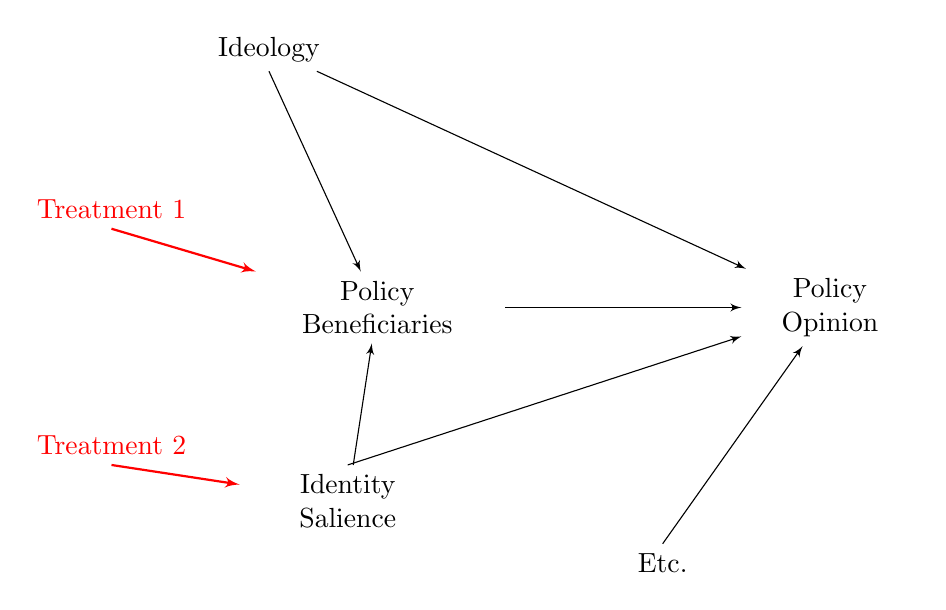
\begin{tikzpicture}[>=latex',circ/.style={draw, shape=circle, node distance=5cm, line width=1.5pt}]
    \draw (0,0) node[left, text width=3cm, align=center] (X) {Policy\\Beneficiaries};
    \draw[->] (X) -- (3,0) node[right, text width=2cm, align=center] (Y) {Policy\\Opinion};
    \draw[->] (-3,3) node[above] (Z) {Ideology} -- (X);
    \draw[->] (Z) -- (Y);
    \draw[->] (2,-3) node[below, text width=3cm, align=center] (E) {Etc.} -- (Y);
    \draw[->] (-2, -2) node[below, text width=2.5cm, align=center] (W) {Identity Salience} -- (Y);
    \draw[->] (W) -- (X);
    \draw<2->[->,thick,red] (-5,1) node[above] (T1) {Treatment 1} -- (X);
    \draw<2->[->,thick,red] (-5,-2) node[above] (T1) {Treatment 2} -- (W);
\end{tikzpicture}
\end{center}
\end{frame}



\frame{
	\frametitle{{\normalsize Ex. Question-as-treatment\footnote{Transue. 2007. ``Identity Salience, Identity Acceptance, and Racial Policy Attitudes: {American} National Identity as a Uniting Force.'' \textit{American Journal of Political Science} 51(1): 78--91.}}}
	

\begin{itemize}
\item \only<1,3>{How close do you feel to your ethnic or racial group?}\only<2,4>{How close do you feel to other Americans?}
\item \only<1-2>{Some people have said that taxes need to be raised to take care of pressing national needs. How willing would you be to have your taxes raised to improve education in public schools?}\only<3-4>{Some people have said that taxes need to be raised to take care of pressing national needs. How willing would you be to have your taxes raised to improve educational opportunities for minorities?}
\end{itemize}
	
}


\frame{

\frametitle{2x2 Factorial Design}

\only<1>{
\begin{center}
\begin{tabular}{lr}
Condition &  \\ \midrule
Educ. for Minorities & $Y_1$ \\
Schools & $Y_0$ \\ \bottomrule
\end{tabular}
\end{center}
}

\only<2>{
\begin{center}
\begin{tabular}{lrr}
Condition & Americans & Own Race \\ \midrule
Educ. for Minorities & $Y_{1,0}$ & $Y_{1,1}$ \\
Schools & $Y_{0,0}$ & $Y_{0,1}$ \\ \bottomrule
\end{tabular}
\end{center}
}

}


\frame{

\frametitle{Two ways to \textit{parameterize} this}

Dummy variable regression (i.e., treatment--control CATEs):

$Y = \beta_0 + \beta_1 X_{0,1} + \beta_2 X_{1,0} + \beta_3 X_{1,1} + \epsilon$

\vspace{1em}

Interaction effects (i.e., treatment--treatment CATEs):

$Y = \beta_0 + \beta_1 X1_{1} + \beta_2 X2_{1} + \beta_3 X1_1 * X2_1 + \epsilon$

\vspace{1em}

Use \texttt{margins} to extract marginal effects

}


\frame<1>[label=factorialconsiderations]{

\frametitle{Considerations}

\begin{itemize}\itemsep0.5em
\item Need to have hypotheses about heterogeneity a priori
\item Factorial designs can quickly become unwieldy and expensive
\item<2-> Need to consider what CATEs are of theoretical interest
	\begin{itemize}
	\item Treatment--control
	\item Treatment--treatment
	\item Marginal effects, averaging across other factors
	\end{itemize}
\end{itemize}

}

\frame{

\frametitle{Probably obvious, but\dots}

\footnotesize

\begin{center}
\begin{tabular}{cccc}
Factors & Conditions per factor & Total Conditions & $n$ \\ \midrule
1 & 2 & 2 & 400 \\ 
1 & 3 & 3 & 600 \\
1 & 4 & 4 & 800 \\
2 & 2 & 4 & 800 \\
2 & 3 & 6 & 1200 \\
2 & 4 & 8 & 1600 \\
3 & 3 & 9 & 1800 \\
3 & 4 & 12 & 2400 \\
4 & 4 & 16 & 3200 \\ \bottomrule
\end{tabular}
\end{center}

{\footnotesize Assumes power to detect a relatively small effect, but no consideration of multiple comparisons.}

}

\againframe{factorialconsiderations}

% marginal effects of factors are marginal across the set of levels of the other factors; if those factors aren't complete, then external validity problem


\questions


\subsubsection{Treatment Self-Selection}

\frame{

\frametitle{Treatment Preferences/Self-Selection}

Bennett and Iyengar:\footnote{p.724 from Bennett \& Iyengar. 2008. ``A new era of minimal effects? The changing foundations of political communication.'' \textit{Journal of Communication} 58(4): 707--31.}

\begin{quote}\small
manipulational control actually weakens the ability to generalize to the real world where exposure to stimuli is typically voluntary. Accordingly, it is important that experimental researchers use designs that combine manipulation with self-selection of exposure.
\end{quote}

}


\frame{

Hovland: \footnote{p.16 from Hovland. 1959. ``Reconciling conflicting results derived from experimental and survey studies of attitude change.'' \textit{American Psychologist} 14(1): 8--17.}

\begin{quote}\small
It should be possible to assess what demographic and personality factors predispose one to expose oneself to particular communications and then to utilize experimental and control groups having these characteristics. Under some circumstances the evaluation could be made on only those who select themselves, with both experimental and control groups coming from the self-selected audience.
\end{quote}

}


\frame{

\frametitle{{\large Treatment Preferences I}}

\begin{itemize}\itemsep0.5em
\item Experiments are about inferring effect of $X$ on $Y$
\item Respondents may have preferences over whether they are treated or untreated\footnote{Rucker. 1989. ``A Two-Stage Trial Design for Testing Treatment, Self-Selection, and Treatment Preference Effects.'' \textit{Statistics in Medicine} 8: 477--485.}
\item Origins of this discussion are in the medical literature\footnote{Swift \& Callahan. 2009. ``The Impact of Client Treatment Preferences on Outcome: A Meta-Analysis.'' \textit{Journal of Clinical Psychology} 65(4): 368--381.}
\item Closely related to the notion of placebo effects
\end{itemize}

}

\frame{

\frametitle{{\large Treatment Preferences I}}

\begin{itemize}\itemsep1em
\item Treatment preferences may be an important factor in:
	\begin{itemize}
	\item Compliance
	\item Effect heterogeneity
	\end{itemize}
\item<2-> Depending on your treatments, you may want to measure preferences
	\begin{enumerate}
	\item<3-> Stated preference measures
	\item<4-> Designs that reveal preferences
	\end{enumerate}
\end{itemize}

}


\frame{

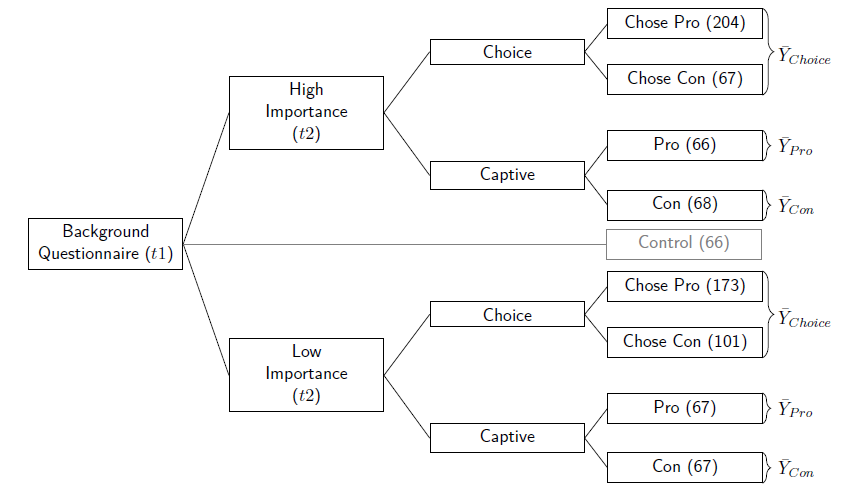
\includegraphics[width=\textwidth]{images/leeper2017}
\vspace{2em}

{\tiny Leeper. 2017. ``How Does Treatment Self-Selection Affect Inferences About Political Communication?'' \textit{Journal of Experimental Political Science}: In Press. Available at \url{http://thomasleeper.com/research.html}\par}

}

\frame{

\frametitle{{\normalsize Analyzing 3-Group Preference Trials\footnote{GK2011 Package for R. \url{https://cran.r-project.org/package=GK2011}}}}

\begin{enumerate}\itemsep0.5em
\item SATE: $\bar{Y}_{T} - \bar{Y}_{C}$
\item CATE (Prefer T): $\dfrac{\bar{Y}_{Choice} - \bar{Y}_{C}}{\hat{\alpha}}$
\item CATE (Prefer C): $\dfrac{\bar{Y}_{T} - \bar{Y}_{Choice}}{1-\hat{\alpha}}$
\end{enumerate}

\vspace{1em}

Note: $\alpha = Pr(T | Choice)$
}



\questions


\subsubsection{Attention and Satisficing}


\frame{

\frametitle{Attention and Satisficing}

One final issue with unit-related sources of heterogeneity is how we handle or analyze survey-experimental data where we think participants ``misbehaved''.

\vspace{1em}

\only<2->{This falls into a couple of broad categories:

\begin{enumerate}
\item Noncompliance (discussed earlier)
\item Survey Satisficing
\item Apparent Inattention
\end{enumerate}
}
}


\frame{
\frametitle{Substantive Manipulation Check}
\begin{itemize}\itemsep1em
\item Two common approaches:
	\begin{itemize}
	\item Information recall or understanding
	\item Measure level of manipulated treatment variable
	\end{itemize}
\item Risky to remove cases based on this because it is a form of conditioning on post-treatment variables
\item May be useful to consider either a mediator of effects
\end{itemize}
}



% attention checks
\frame{
\frametitle{Attention Checking}

\large 
\begin{itemize}\itemsep1em
\item Online mode invites satisficing
\item Attention checking can help, but is imperfect
\end{itemize}
}

% useful for checking attention
% may have consequences for representativeness and introduce selection biases

\frame{
\frametitle{Apparent Satisficing}
\begin{itemize}\itemsep0.5em
\item Filter out respondents based on response behavior
\item Some common measures:
	\begin{itemize}
	\item ``Straightlining''
	\item Non-differentiation
	\item Acquiescence
	\item Nonresponse
	\item DK responding
	\item Speeding
	\end{itemize}
\item Difficult to detect
\item Difficult to distinguish from ``real'' responses
\end{itemize}
}

\frame{
\frametitle{Metadata/Paradata}
\begin{itemize}\itemsep1em
\item<1-> Timing
	\begin{itemize}
	\item Some survey tools will allow you to time page
	\item Make a prior rules about dropping participants for speeding
	\end{itemize}
\item<2-> Mousetracking or eyetracking
	\begin{itemize}
	\item Mousetracking is unobtrusive
	\item Eyetracking requires participants opt-in
	\end{itemize}
\item<3-> Record focus/blur browser events
\end{itemize}
}

\frame{
\frametitle{Direct Measures}
\begin{itemize}\itemsep2em
\item How closely have you been paying attention to what the questions on this survey actually mean?
\item<2-> While taking this survey, did you engage in any of the following behaviors? Please check all that apply.
	\begin{itemize}
	\item Use your mobile phone
	\item Browse the internet
	\item \dots
	\end{itemize}
\end{itemize}
}


\frame{
\frametitle{Instructional Manipulation Check}

\only<2>{Do you agree or disagree with the decision to send British forces to fight ISIL in Syria? }We would like to know if you are reading the questions on this survey. If you are reading carefully, please ignore this question, do not select any answer below, and click ``next'' to proceed with the survey.\\

\vspace{1em}

\small

Strongly disagree\\
Somewhat disagree\\
Neither agree nor disagree\\
Somewhat agree\\
Strongly agree\\

}


\frame{
\frametitle{Attention Checking}

In summary\dots

\begin{itemize}\itemsep1em
\item Attention checking can be useful
\item Lots of options
\item No obvious best metric
\item Can be analytically consequential
\end{itemize}
}







\frame{

How should we deal with respondents that appear to not be paying attention, not ``taking'' the treatment, or not responding to outcome measures?

\begin{enumerate}
\item Keep them
\item Throw them away
\end{enumerate}

}

\frame{

\frametitle{Best Practice: Protocol}

\begin{itemize}\itemsep0.5em
\item Excluding respondents based on survey behavior is one of the easiest ways to ``p-hack'' an experimental dataset
	\begin{itemize}
	\item Inattention, satisficing, etc. will tend to reduce the size of the SATE
	\end{itemize}
\item So regardless of how you handle these respondents, these should be decisions that are made \textit{pre-analysis}
\end{itemize}

}


\frame[label=exclusion]{

\frametitle{{\normalsize When are you excluding participants?}}

    \begin{columns}[T]
    \begin{column}[T]{5cm}
        \begin{block}{\rule[-0.6ex]{0pt}{2.5ex}Pre-Treatment}
            \begin{itemize}\itemsep0.2em
                \item<2-> \hyperlink{satisficing}{Satisficing behaviors}
                \item<3-> Inattention
                \item<4-> Covariate-based selection
                \item<5-> Pretreated
            \end{itemize}
        \end{block}
    \end{column}
    \begin{column}[T]{5cm}
        \begin{block}{\rule[-0.6ex]{0pt}{2.5ex}Post-Treatment}
            \begin{itemize}\itemsep0.5em
                \item<6-> Speeding on treatment
                \item<7-> ``Failing'' a manipulation check
                \item<8-> Drop-off
            \end{itemize}
        \end{block}
    \end{column}
    \end{columns}

}


\frame{

\frametitle{Pre-Treatment Exclusion}

\begin{itemize}\itemsep0.5em
\item This is totally fine from a causal inference perspective
\item<2-> Advantages:
	\begin{itemize}
	\item Focused on engaged respondents
	\item Likely increase impact of treatment
	\end{itemize}
\item<3-> Disadvantages:
	\begin{itemize}
	\item Changing definition of sample (and thus population)
	\end{itemize}
\end{itemize}

}




\frame{

\frametitle{Post-Treatment Exclusion}

This is much more problematic because it involves controlling for a \textit{post-treatment} variable

}

\frame<1-3>[label=posttreatment]{

\begin{center}
\begin{tikzpicture}[>=latex',circ/.style={draw, shape=circle, node distance=5cm, line width=1.5pt}]
    \draw (0,0) node[left, text width=3cm, align=center] (X) {Information};
    \draw (5,0) node[right, text width=2cm, align=center] (Y) {Opinion};
    \draw<1-3>[->] (X) -- (Y);
    \draw[->] (4,-4) node[below, text width=3cm, align=center] (E) {Etc.} -- (Y);
	\draw<2-> (1,-2) node[text width=3cm, align=center] (M) {Manipulation Check};
	\draw<2-4>[->,thick,red] (X) -- (M);
    \draw<2-4>[->,thick,red] (M) -- (Y);
    \draw<3>[->] (E) -- (M);
\end{tikzpicture}
\end{center}

\small 
\only<2>{Risk that estimate of $\beta_1$ is diminished because effect is being carried through the manipulation check.}
\only<3>{Introduction of ``collider bias'' wherein values of the manipulation check are affected by other factors.}
}





\frame[label=posttreatment2]{

\frametitle{Post-Treatment Exclusion}

\small

\begin{itemize}\itemsep0.5em
\item Any post-treatment exclusion is problematic and should be avoided
\item<2-> Can estimate a LATE
	\begin{itemize}\footnotesize
	\item Interpretation: Effect of manipulation check among those whose value of the check can be changed by the treatment manipulation
	\end{itemize}
\item<3-> Non-response or attrition is the same as researcher-imposed exclusion
	\begin{itemize}\footnotesize
	\item Not problematic if MCAR
	\item Nothing really to be done if caused by treatment
	\end{itemize}
\end{itemize}

}

\againframe<3-4>{posttreatment}

\againframe<2->{posttreatment2}


\frame{}

% Talk about protocol and preregistration

\frame{

\frametitle{Protocol}

Protocol is the complete planning document for how to design, implement, and analyze an experiment.\footnote{Thomas J. Leeper. 2011. ``The Use of Protocol in the Design and Reporting of Experiments.'' \textit{The Experimental Political Scientist}.}

}

\frame{

\frametitle{{\normalsize Protocol}}


\small

\begin{enumerate}\itemsep-0.2em
\item Theory/hypotheses
\item Instrumentation
	\begin{itemize}
	\item Manipulation(s)
	\item Outcome(s)
	\item Covariate(s)
	\item Manipulation check(s)
	\end{itemize}
\item Sampling
\item Implementation
\item Analysis
\end{enumerate}
}

\frame{

\frametitle{Why bother?}

\begin{itemize}\itemsep0.5em
\item<2-> Be clear to yourself what you're trying to do before you do it
\item<3-> Assess the literature for best practices
\item<4-> Highlight areas in need of pilot testing
\item<5-> Economize questionnaire development
\item<6-> Study preregistration
\end{itemize}

}

\questions



\questions





\subsection[T]{Treatments}

\frame{

\frametitle{Heterogeneity due to \textit{T}reatments}

\begin{itemize}\itemsep1em
\item We should expect this! Why?
\item<2-> What can we do?
	\begin{itemize}
	\item Pilot testing
	\item Replication
	\item More complex design
	\item Conjoint experiments
	\end{itemize}
\end{itemize}

}



\frame{

\frametitle{Conjoint Designs I}

\small

\begin{itemize}
\item ``Classic vignettes'' taken to an extreme
	\begin{itemize}
	\item Address heterogeneity w/r/t SU\textbf{T}O
	\end{itemize}
\item Example: Judge whether to admit an immigrant to your country
\item<2-> Respondents see a series of vignettes that are fully randomized along any number of dimensions
	\begin{itemize}\footnotesize
	\item Sex, Education, Language proficiency, etc.
	\end{itemize}
\item<3-> Outcome is judgment (binary or rating scale)
\end{itemize}

}

\frame{

\frametitle{Conjoint Designs II}

Why is this useful?

\begin{itemize}\itemsep0.5em
	\item Understand complex decision-making
	\item Within-subjects comparisons
	\item Heterogeneous effects across versions of treatment
	\item Pilot testing: Sensitivity of design to specification of \textit{compound} vignette
\end{itemize}

}


\frame{
\begin{center}
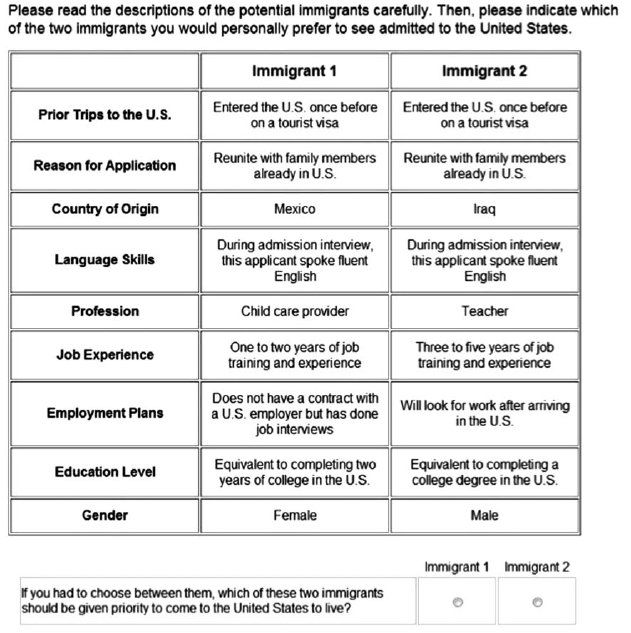
\includegraphics[height=\textheight]{images/conjoint1}
\end{center}
}

\frame{
\begin{center}
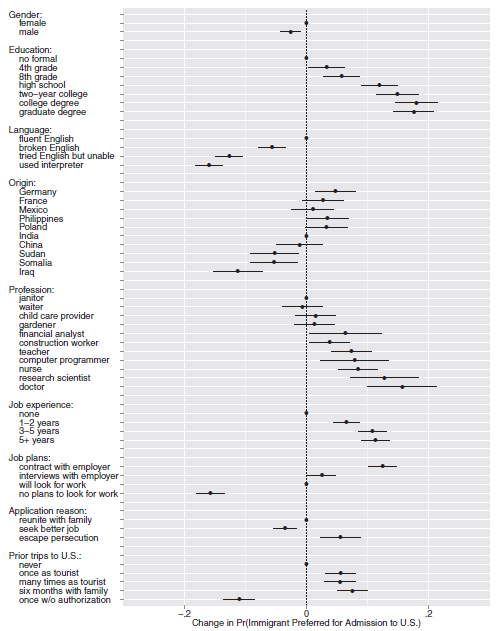
\includegraphics[width=\textwidth]{images/conjoint2}
\end{center}
}

\frame{

\frametitle{Conjoint Designs III}


\begin{itemize}\itemsep0.5em
\item<2-> As long as profiles are randomized, this is just a complex factorial design where we can estimate \textit{marginal effect} of each attribute
	\begin{itemize}\footnotesize
	\item Treatment--control SATE, conditional on all other randomized factors
	\end{itemize}
\item<3-> Assumptions:
	\begin{itemize}\footnotesize
	\item Fully randomized profiles
	\item No ``carry-over'' effects
	\item No profile order effects
	\end{itemize}
\end{itemize}

}


\frame{}

\frame{

\frametitle{Replication}

\begin{itemize}\itemsep1em
\item Conjoints solve one problem: they identify the relative size of sources of heterogeneity within a given treatment
\item<2-> But how should we consider experiments testing the same theory using different treatments?
	\begin{itemize}
	\item ``Triangulation''
	\item Consistent directionality
	\item Consistent (standardized) effect sizes
	\end{itemize}
\item<3-> Big conclusion: replication is important and there's not enough of it.
\end{itemize}
}

\questions



\subsection[O]{Outcomes}

\frame{

\frametitle{Heterogeneity due to \textit{O}utcomes}

\begin{itemize}\itemsep1em
\item This is expected!
	\begin{itemize}
	\item E.g., non-equivalent outcomes
	\end{itemize}
\item Reasonable to explore multiple outcomes
	\begin{itemize}
	\item Multiple comparisons
	\item Power considerations
	\item Construct validity
	\end{itemize}
\item<2-> What outcomes you measure depend on your theory
\item<3-> Lots of potential for behavioral measures!
\end{itemize}

}


\frame{
\frametitle{Behavioural measures}
Some behaviours that can be directly measured through survey questionnaires.

\vspace{1em}

\only<2->{Three broad categories:}
\begin{enumerate}
\item<3-> Behavioural measures that provide survey paradata % (response latency, reading times, answer switching, nonresponse)
\item<4-> Behavioural measures that operationalize attitudes % IAT
\item<5-> Behavioural measures that operationalize behaviours % (e.g., political participation; purchasing)
\end{enumerate}
}


\frame{
\frametitle{Behavioural Measures for Paradata}

Why?
	\begin{itemize}
	\item Respondents use of the survey tells us something meaningful about their behaviour
	\end{itemize}
\only<2->{What?
	\begin{itemize}
	\item<3-> Nonresponse
	\item<4-> Response latencies
	\item<5-> Reading times
	\item<6-> Answer switching
	\item<7-> Eye tracking
	\item<8-> Mouse tracking
	\item<9-> Smartphone metadata
	\end{itemize}
}
}


\frame{
\frametitle{Behavioural Measures for Attitudes}

Why?
	\begin{itemize}
	\item Attitudinal self-reports might be ``cheap talk''
	\end{itemize}

\vspace{1em}
\only<2->{What?
	\begin{itemize}
	\item<3-> Implicit Association Test
	\item<4-> Incentivized Survey questions
	\end{itemize}
}
}



\frame{

\frametitle{Behavioural Measures for Behaviour}

Why?
	\begin{itemize}
	\item We want to observe or affect behaviour (e.g., in an experiment)
	\end{itemize}
	
\vspace{1em}
\only<2->{What? 
	\begin{itemize}
	\item Directly measure or initiate a direct measure of a behaviour
	\item May be measured by something that occurs within the confines of the survey or something outside of the survey
	\end{itemize}
}
}


\frame<1-2>[label=infochoice]{

\frametitle{Example 1:\\Active Information Choice}

\begin{itemize}\itemsep0.5em
\item<2-> ``Followed link'' identification\footnote{Guess, AM. 2015. ``Measure for Measure.'' \textit{Political Analysis} 23: 59--75. \href{http://doi.org/10.1093/pan/mpu010}{doi:10.1093/pan/mpu010} }

\item<3-> Information boards\footnote{Leeper, TJ. 2014. ``The Informational Basis for Mass Polarization.'' \textit{Public Opinion Quarterly} 78(1): 27--46. \href{http://doi.org/10.1093/poq/nft045}{doi:10.1093/poq/nft045}}

\item<4-> Video choice\footnote{Arceneaux, K \& Johnson, M. 2012. \textit{Changing Minds or Changign Channels}. Chicago: The University of Chicago Press.}

\item<5-> Dynamic Process Tracing Environment \footnote{\url{https://dpte.polisci.uiowa.edu/dpte/}}
\end{itemize}

}

\frame{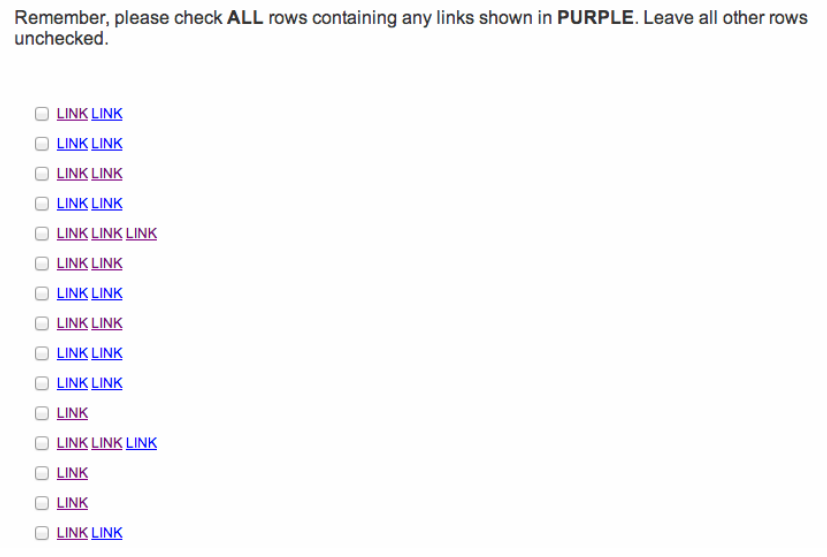
\includegraphics[width=\textwidth]{images/linksguess.png}}

\againframe<2-3>{infochoice}

\frame{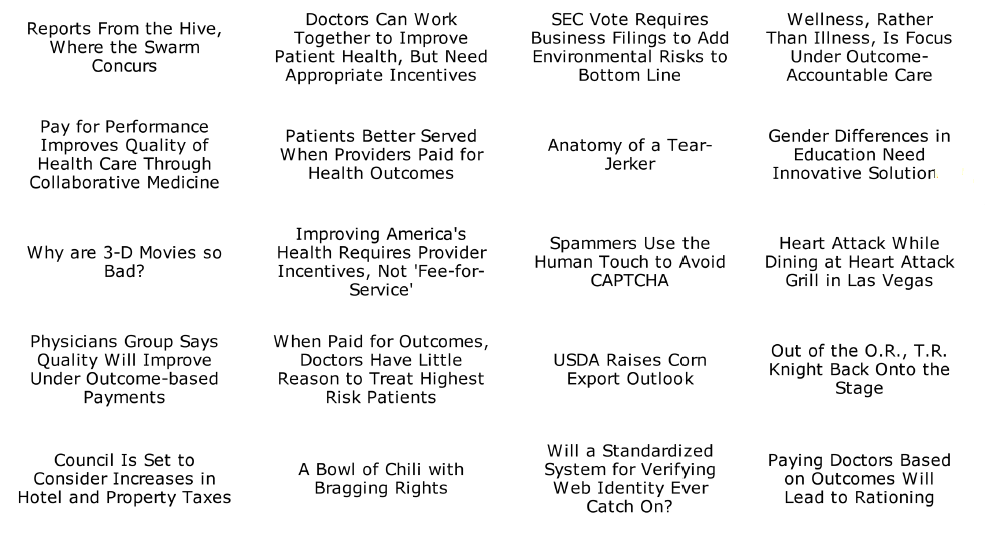
\includegraphics[width=\textwidth]{images/leeper.png}}

\againframe<3-5>{infochoice}

\frame{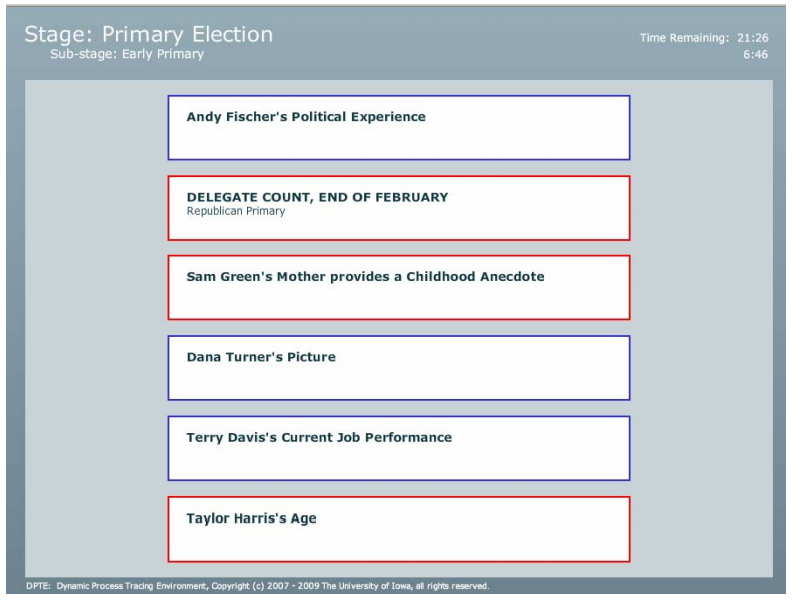
\includegraphics[width=\textwidth]{images/dpte1.png}}
\frame{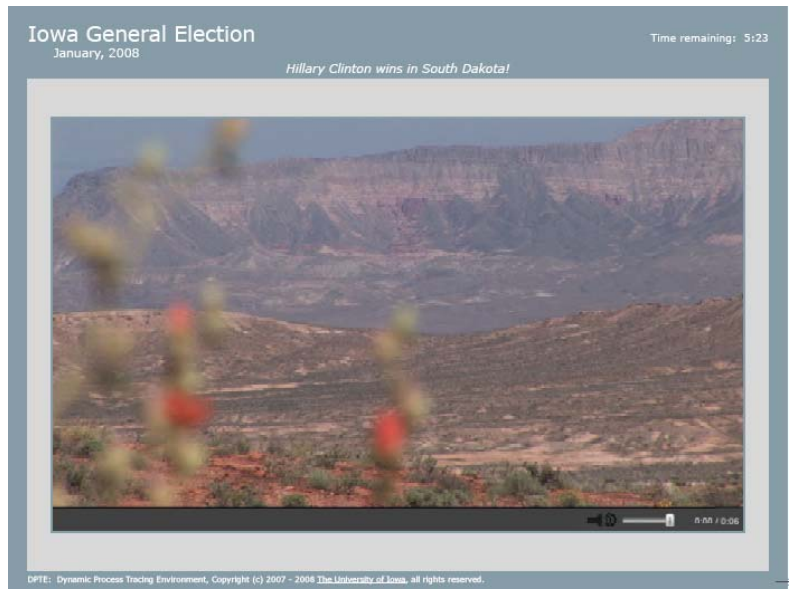
\includegraphics[width=\textwidth]{images/dpte2.png}}
\frame{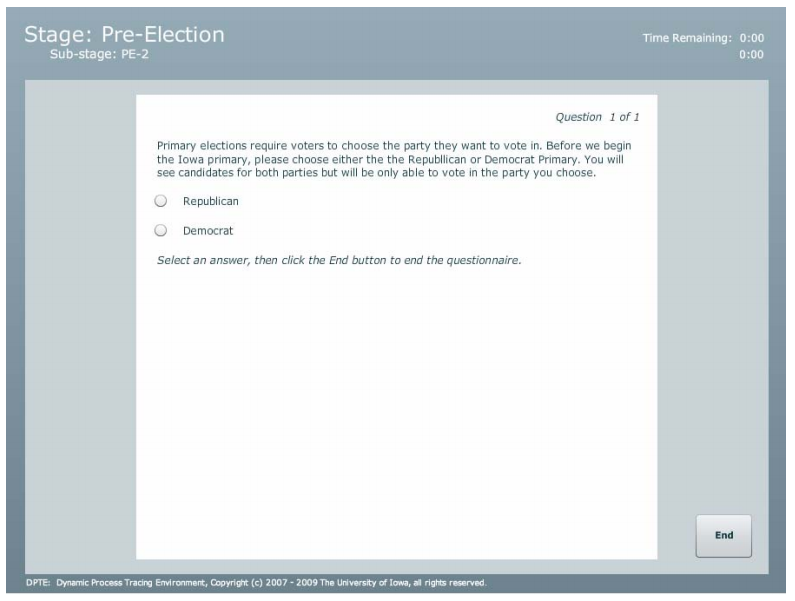
\includegraphics[width=\textwidth]{images/dpte3.png}}



\frame{

\frametitle{Example 2:\\Sign-up/Enrolment}

An extension of information choice behaviour would be explicit engagement in other kinds of (small) behaviours, such as:

\begin{itemize}\itemsep0.5em
\item Entering an email address to receive information or join a mailing list \footnote{Leeper, TJ. 2017. ``How Does Treatment Self-Selection Affect Inferences About Political Communication?'' \textit{Journal of Experimental Political Science}: In press.} \footnote{Bolsen, Druckman, \& Cook. 2014. ``Communication and Collective Actions.'' \textit{Journal of Experimental Political Science} 1(1): 24--38. \href{http://doi.org/10.1017/xps.2014.2}{doi:10.1017/xps.2014.2}}

\item Signing up for an appointment or further interaction
\end{itemize}

}


\frame<1>[label=incentivised]{
\frametitle{Example 3:\\Incentivised Survey Questions}

Definitions:

\begin{itemize}\itemsep0.5em
\item A survey question is just a self-report
\item An \textit{incentivized} survey question attached financial gains or losses to the answer options
\end{itemize}

\vspace{1em}
\only<2->{
Paradigm could be applied to any measure of behavioural intentions to avoid cheap talk.
}

}

\frame{

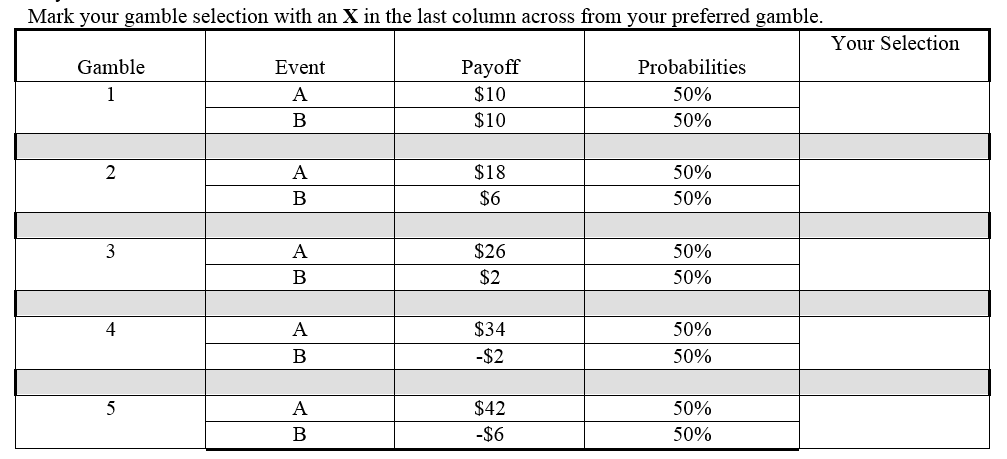
\includegraphics[width=\textwidth]{images/eckelgrossman.png}

\vspace{2em}
{\tiny Eckel \& Grossman. 2008 ``Forecasting risk attitudes.'' \textit{Journal of Economic Behavior \& Organization} 68(1): 1--17. \href{http://doi.org/10.1016/j.jebo.2008.04.006}{doi:10.1016/j.jebo.2008.04.006}\par }
}

\againframe<1->{incentivised}


\frame[label=purchasing]{
\frametitle{Example 4:\\Purchasing Decisions}

Common ways to study purchasing behaviour include:

\begin{itemize}
\item<2-> Direct attitudinal questions
\item<3-> Retrospective and prospective self-reports
\item<4-> Conjoint experiments
\end{itemize}

\only<5->{Another way is embedding a purchase in a survey.\footnote{Bolsen, T. 2011. ``A Lightbulb Goes On.'' \textit{Political Behavior} 35(1): 1--20.  \href{http://doi.org/10.1007/s11109-011-9186-5}{10.1007/s11109-011-9186-5}
}}

}

\frame{

\begin{center}
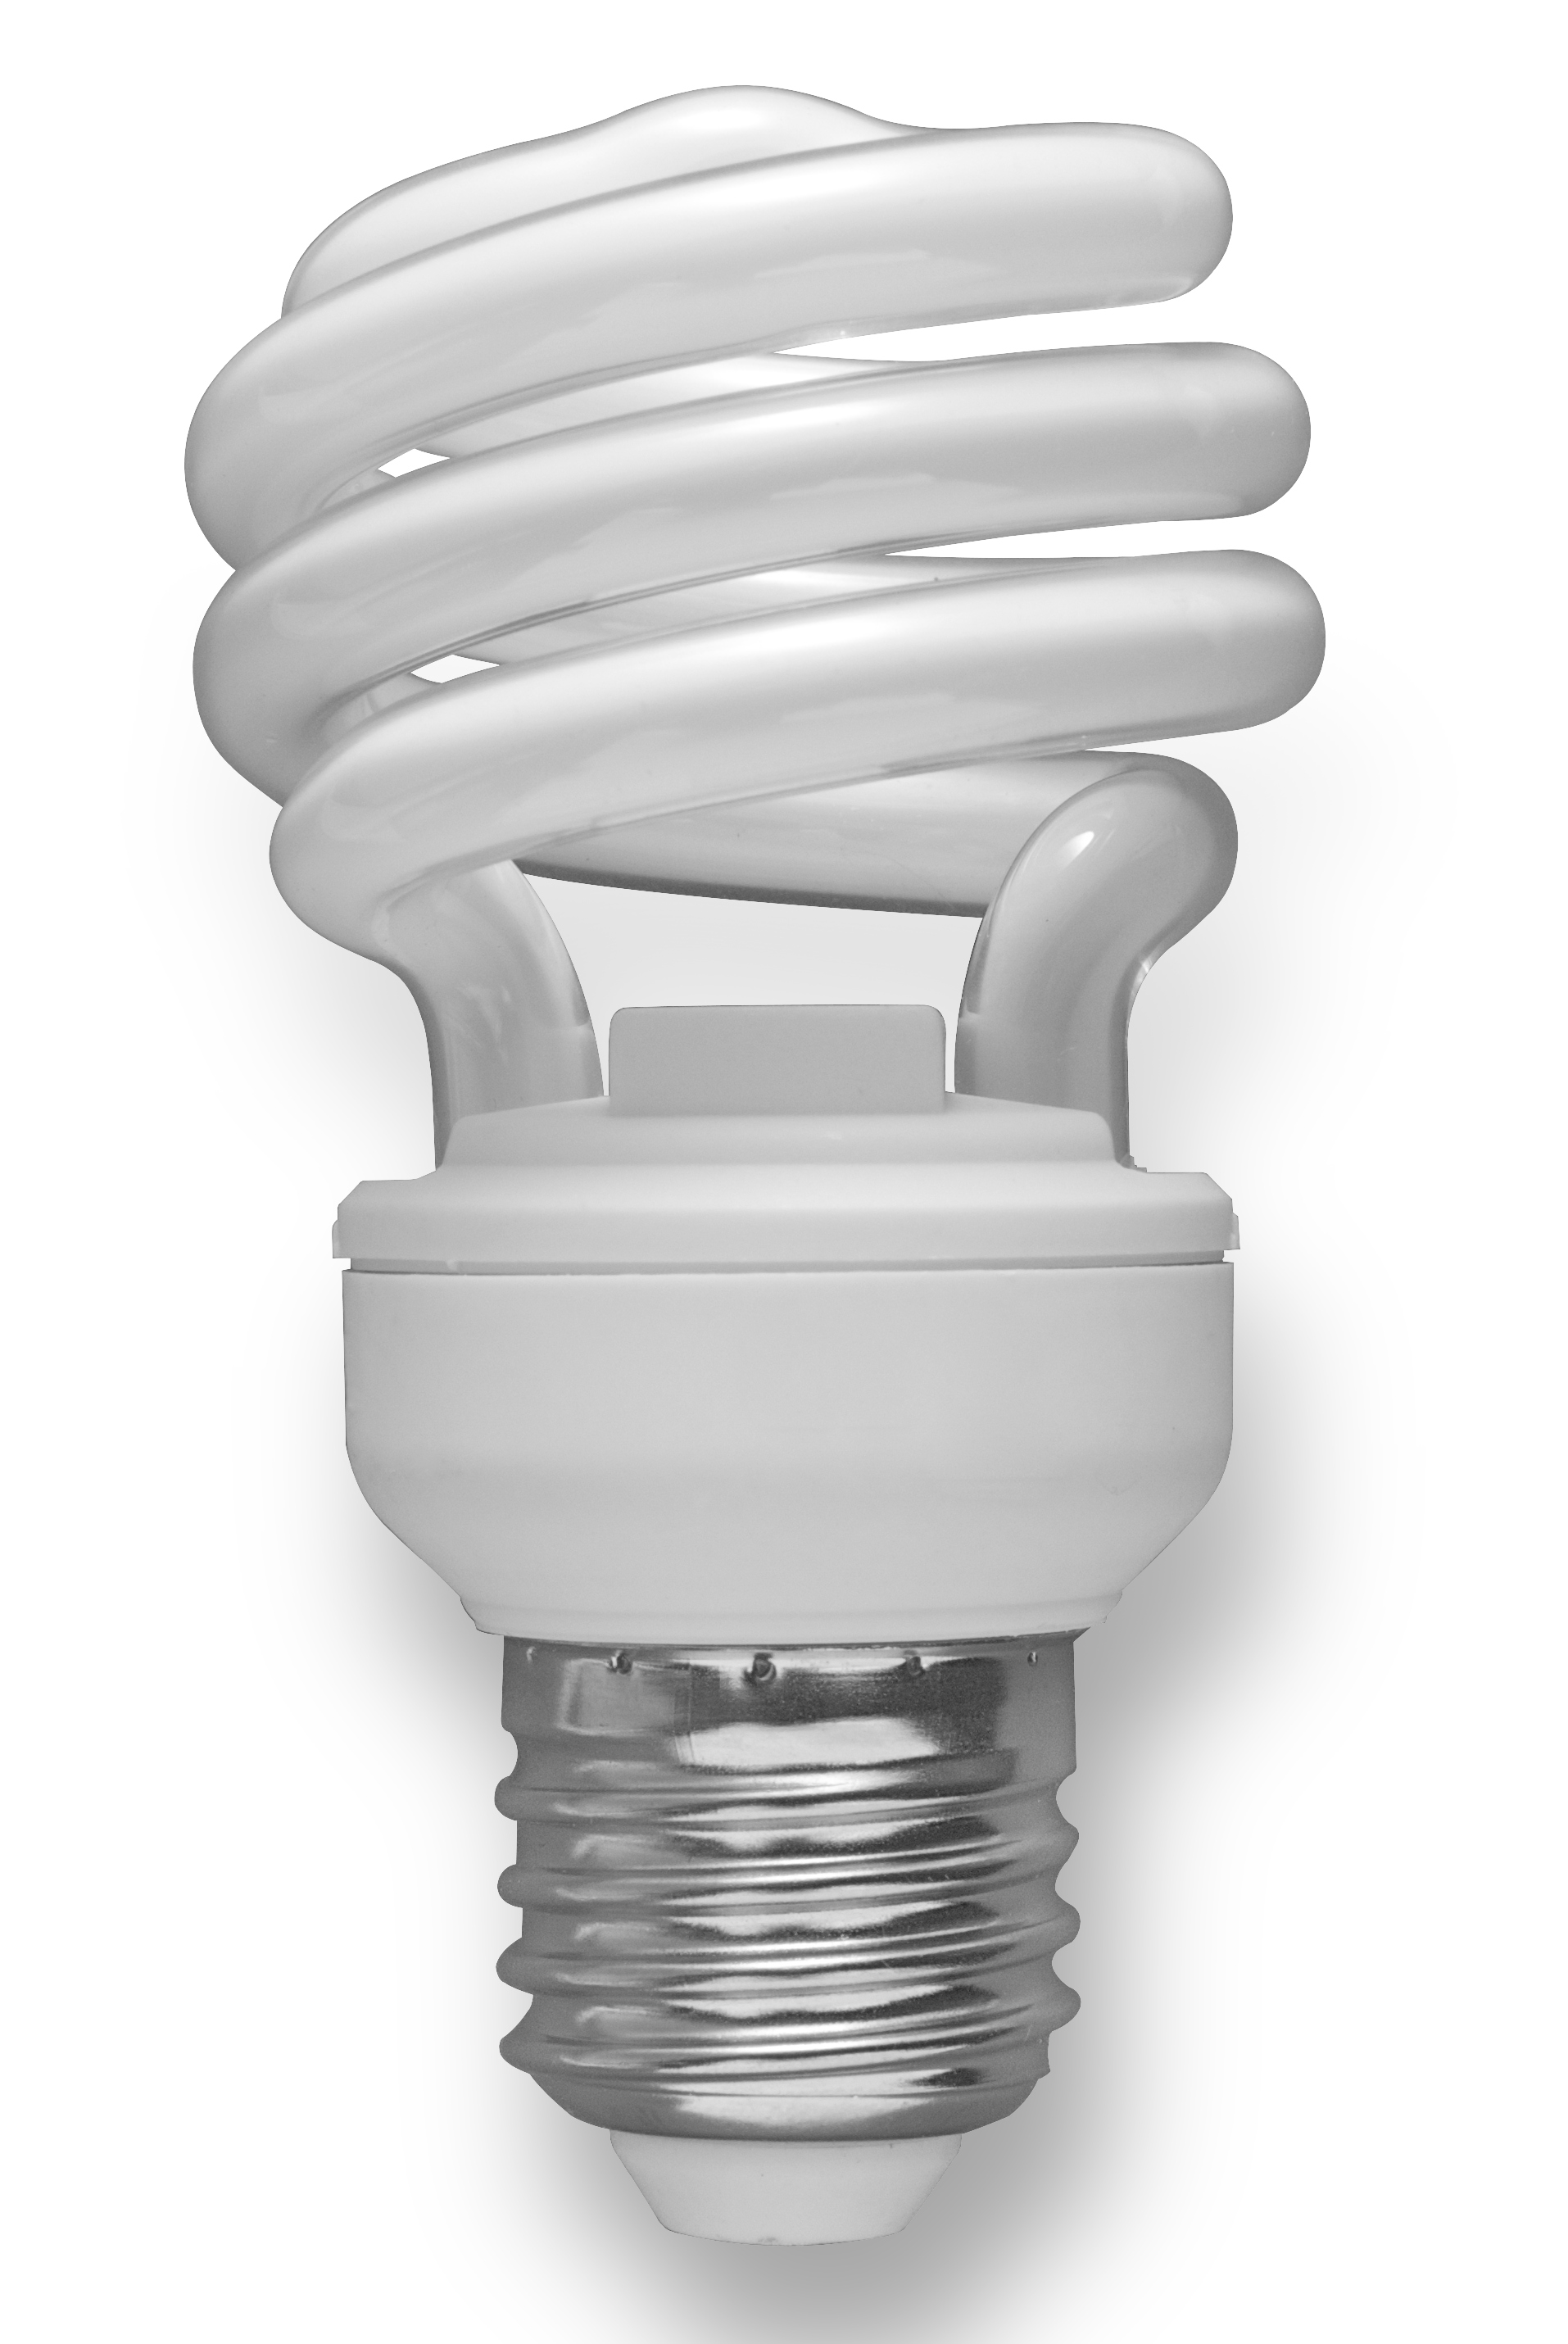
\includegraphics[width=.45\textwidth]{images/lightbulb1.png}
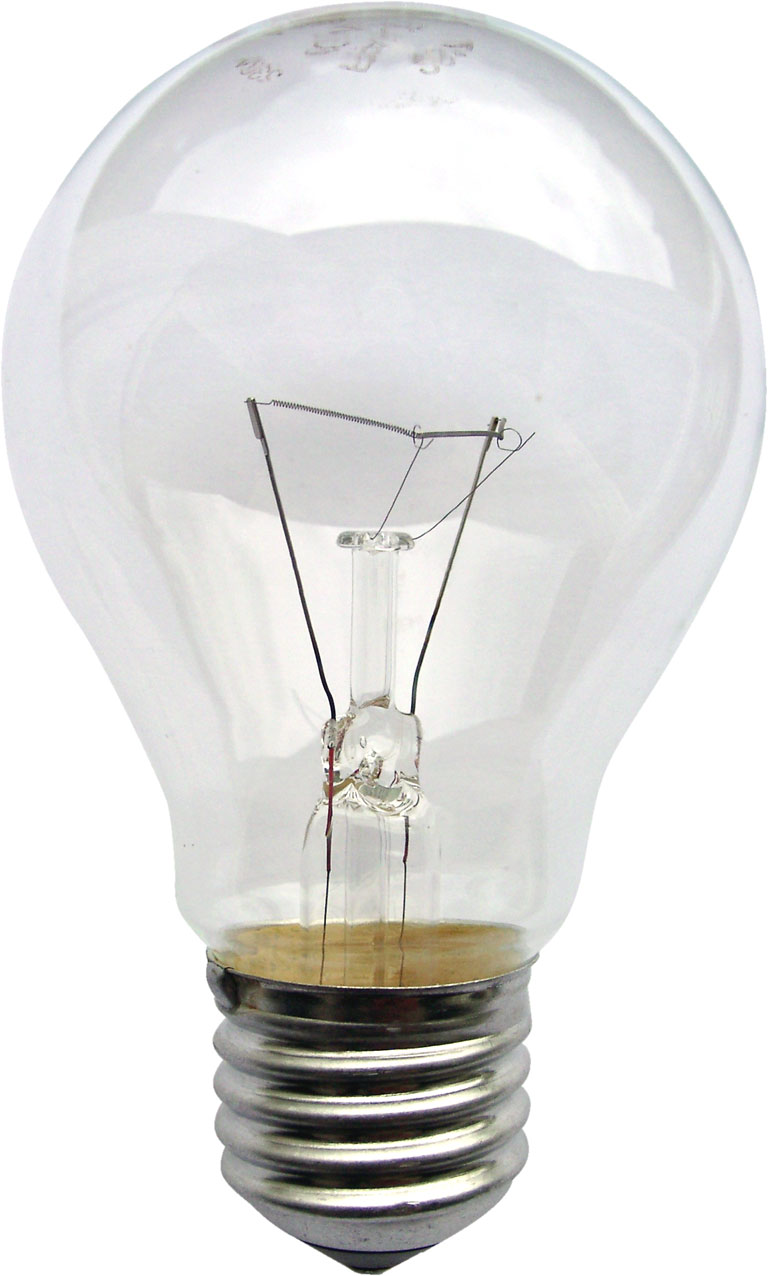
\includegraphics[width=.38\textwidth]{images/lightbulb2.png}
\end{center}

\vspace{1em}

{\tiny 
Source: Wikimedia Commons (\href{https://commons.wikimedia.org/wiki/File:06_Spiral_CFL_Bulb_2010-03-08_(white_back).jpg}{Sun Ladder}, \href{https://commons.wikimedia.org/wiki/File:Gluehlampe_01_KMJ.jpg}{KMJ}) \par }

}


\frame{

\frametitle{Example 5:\\Donations}

\begin{itemize}\itemsep1em
\item Miller and Krosnick\footnote{Miller, Krosnick, \& Lowe. N.d. ``The Impact of Policy Change Threat on Financial Contributions to Interest Groups.'' Working paper.} asked for charitable donations via cheque directly as part of a paper-and-pencil survey

\item<2-> Klar and Piston\footnote{Klar \& Piston. 2015. ``The influence of competing organisational appeals on individual donations.'' \textit{Journal of Public Policy} 35(2): 171--91. \href{http://doi.org/10.1017/S0143814X15000203}{doi:10.1017/S0143814X15000203}} offered respondents a survey incentive up-front for participation and then later offered them a chance to donate (a portion of payment) to a charity
\end{itemize}

}




\frame{

\frametitle{Example 6:\\Web Tracking Data}

\begin{enumerate}\itemsep1em
\item Active installation of a tracking app, such as YouGov Pulse\footnote{\url{https://yougov.co.uk/find-solutions/profiles/pulse/}} \footnote{Guess, AM. N.d. ``Media Choice and Moderation.'' Working paper, \url{https://dl.dropboxusercontent.com/u/663930/GuessJMP.pdf}.}

\item Post-hoc collection of web history files using something like Web Historian \footnote{\url{http://www.webhistorian.org/}}
\end{enumerate}
}



\frame<1-2>[label=other]{
\frametitle{Other Possibilities}

\begin{itemize}\itemsep1em
\item<2-> Coordination tasks
	\begin{itemize}
	\item Synchronous group tasks\footnote{Mao, Mason, Suri, Watts. 2016. ``An Experimental Study of Team Size and Performance on a Complex Task.'' \textit{PLoS ONE} 11(4): e0153048. \href{http://doi.org/10.1371/journal.pone.0153048}{doi:10.1371/journal.pone.0153048}} 
	\item Game play
	\item Simulations
	\end{itemize}
\item<3-> Offering incentives to perform future behaviour (tracked elsewhere)
\item<4-> OAuth/API integrations w/ other platforms
	\begin{itemize}
	\item Merging website usage data w/ survey data
	\item Treating website sign-up or usage as behavioural outcomes
	\item Linking with smartphone metadata
	\end{itemize}
\end{itemize}
}

\frame{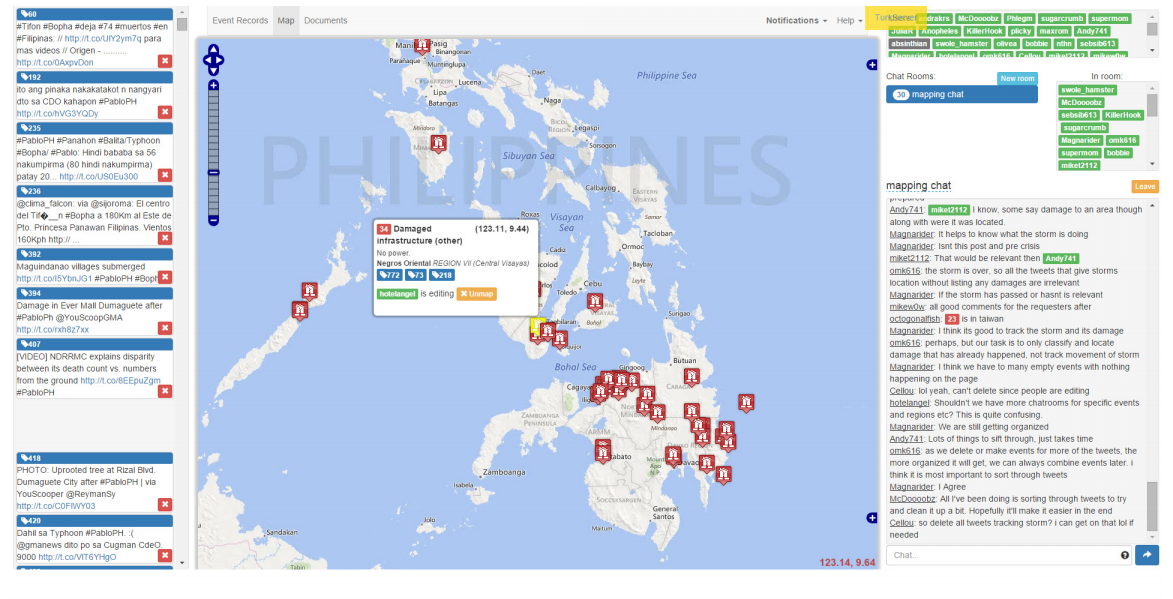
\includegraphics[width=\textwidth]{images/mao.png}}


\againframe<2->{other}


\frame{}

\frame{

\frametitle{Some principles for survey measures of behaviour}

\begin{enumerate}\itemsep1em
\item<2-> Know why you are collecting a behavioural measure!
\item<3-> Know whether you are studying a past, present, or future behaviour.
\item<4-> Be creative! Recognise possibilities and limitations of any given survey mode.
\item<5-> Validate, validate, validate!
\end{enumerate}

}

\frame{

\frametitle{Activity!}

\large 

\begin{center}
With a partner, brainstorm how one or more these behavioural measures might be applied to a survey experiment (either as outcome, treatment, covariate, or behavioural check) relevant to your own work or your organisation.
\end{center}

}




\frame{}

\frame{

\frametitle{\textit{SUTO} Punchline 1: Replication!}

\small

\begin{itemize}\itemsep0.5em
\item If we think effects are homogeneous (across SUTO), then replications in other SUTO conditions should provide us the same SATE (within sampling error)
\item If we think effects are heterogeneous, then replications should give \textit{systematically} different SATE (or CATE) estimates
	\begin{itemize}\footnotesize
	\item<2-> Identify those patterns of heterogeneity using meta-analysis
	\item<3-> Regress effect estimates from multiple studies on SUTO features of each study
	\end{itemize}
\end{itemize}

}

\frame{}


\frame{

\frametitle{\textit{SUTO} Punchline 2:\\What do you want to know?}

\begin{itemize}\itemsep0.5em
\item Do we want to know SATE, CATE(s), or both?
\item<2-> Decide in advance
	\begin{itemize}
	\item Include in protocol
	\item Design study to estimate CATE(s)
	\end{itemize}
\item<3-> Estimation of unit-related CATEs
	\begin{itemize}
	\item Block randomization
	\item Post-hoc procedures
	\end{itemize}
\end{itemize}

}


\questions



\section[Recruitment]{Participant Recruitment}
\frame{\tableofcontents[currentsection,subsubsectionstyle=hide]}


\frame{
\frametitle{Recruitment Considerations}
\begin{itemize}
\item Recruitment
	\begin{itemize}
	\item Sampling
	\item Opt-in
	\item A mix of each
	\end{itemize}
\item Incentives
\item Frequency of participation
	\begin{itemize}
	\item MTurk panelists do 100+ studies per month
	\item YouGov panelists do nearly as many
	\end{itemize}
\item ``Profile'' variables
\item Quotas, post-stratification, weighting
\item Respondent ``quality''
\end{itemize}
}


\frame{
\frametitle{Professional Panels}
\begin{itemize}\itemsep1em
\item Big players: SSI, YouGov, GfK, TNS/Gallup
\item Online panels of respondents
\item Respondents participate for incentives
\item Study costs are negotiated
	\begin{itemize}
	\item Sample size
	\item Study length (number of survey items)
	\item Targeting
	\item Timing
	\end{itemize}
\end{itemize}
}



\frame{
\frametitle{Opt-in (Crowdsourcing) Sites}
\begin{itemize}\itemsep1em
\item Not exactly a panel (fully opt-in)
\item Incentivized participation
\item<2-> Prominent examples
	\begin{itemize}
	\item MTurk
	\item Crowdflower
	\item Microworkers
	\item Prolific Academic
	\item Google Surveys
	\end{itemize}
\end{itemize}
}


\frame{
\frametitle{``River Sampling''}
\begin{itemize}\itemsep1em
\item Not using an existing subject pool
	\begin{itemize}
	\item Link sharing or posting on websites
	\item Using email list
	\item Online advertising (Google, Facebook)
	\end{itemize}
\item<2-> My advice: don't do this unless you have no other choice!
\end{itemize}
}

\frame{
\frametitle{Custom Panels}
\begin{itemize}\itemsep1em
\item Creating your own panel is great
	\begin{itemize}
	\item Carefully sample on specific characteristics % stanford model; qualification model; database model
	\item Organize repeated interviewing or interaction
	\end{itemize}
\item Lots of additional issues
	\begin{itemize}
	\item Attrition
	\item Compensation
	\item Panel Conditioning
	\end{itemize}
\item See Callegaro et al. 2014. \textit{Online Panel Research: A Data Quality Perspective}. Wiley.
\end{itemize}
}


\frame{
\frametitle{My Advice, Elaborated}
\begin{itemize}\itemsep1em
\item Only work with populations where each unit is uniquely identifiable
\item<2-> Without this, you risk many things:
	\begin{itemize}
	\item Ambiguous eligibility
	\item Retakes, treatment crossover
	\item No way to evaluate response rates/bias
	\end{itemize}
\item<3-> Know something about your sample
	\begin{itemize}
	\item How does it differ from your target of inference?
	\item What theories or evidence would suggest those differences should matter?
	\item What can you do to adjust or control for those \textit{consequential} differences?
	\end{itemize}
\end{itemize}
}



\frame{
\frametitle{Measure, Measure, Measure}

\vspace{1em}

The only way to evaluate a sample is to know something about it.

\vspace{1em}

The best way to convince reviewers is to rule out irrelevancies.
}


\frame{
\frametitle{Don't forget statistical power\dots}
\begin{center}
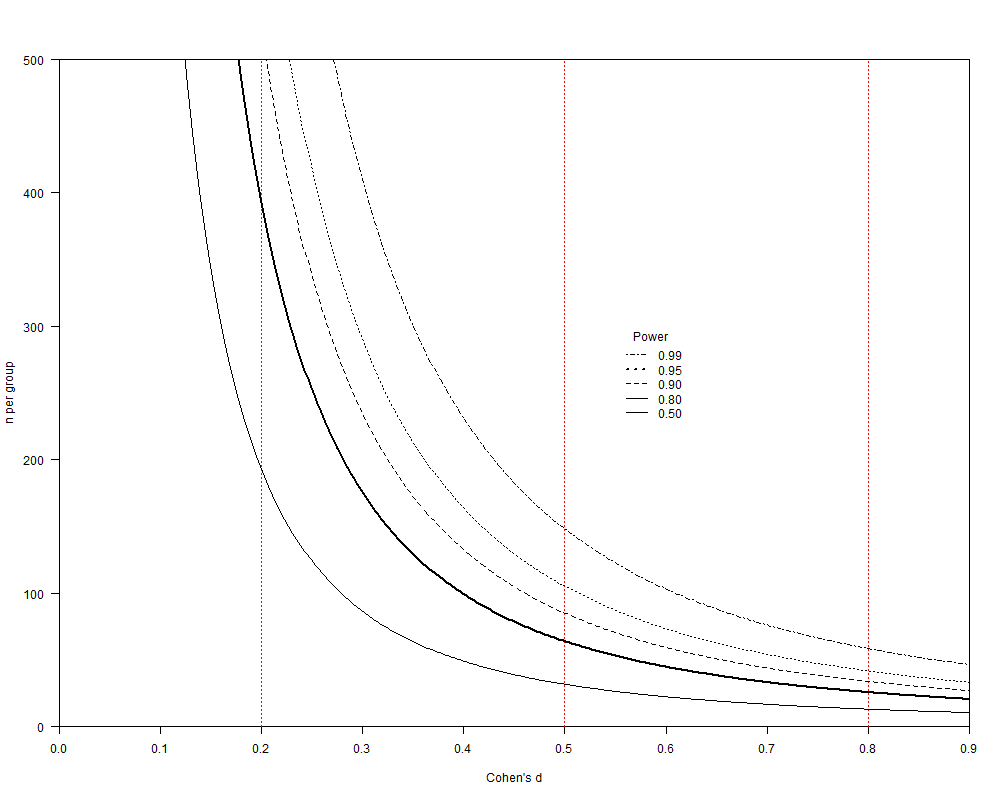
\includegraphics[height=0.85\textheight, trim = 0in 0in 0in 0.5in , clip]{images/power}
\end{center}
}

\frame{
\frametitle{And don't forget costs, either!}

From one of my studies:\\

\vspace{1em}

\centering
\begin{tabular}{l r r r}
Sample	& Cost	& n	& Cost/participant\\ \midrule
National	& \$13200	& 593	& \$22.26\\
Exit Poll	& \$3000	& 741	& \$4.05\\
Students	& \$0	& 299	& \$0\\
Staff		& \$1280	& 128	& \$10.00\\
MTurk	& \$550	& 1024	& \$0.54\\
Ads		& \$636	& 80		& \$7.95\\
\bottomrule
\end{tabular}
}


\frame{}

\appendix
\frame{}

\end{document}
